\documentclass[a4paper, answers, addpoints, 11pt]{exam}
%\documentclass{article}
\addtolength{\hoffset}{-1.25cm}
\addtolength{\textwidth}{2.75cm}
\addtolength{\voffset}{-2.0cm}
\addtolength{\textheight}{3cm}
\setlength{\parskip}{0pt}
\setlength{\parindent}{0in}


%----------------------------------------------------------------------------------------
%	PACKAGES AND OTHER DOCUMENT CONFIGURATIONS
%----------------------------------------------------------------------------------------
\usepackage{amsmath}   % For mathematical formatting and equations
\usepackage{amsthm, amsmath, amssymb} % Mathematical typesetting
\newtheorem{definition}{Definición}
\newtheorem{theorem}{Teorema}
\newtheorem{lemma}{Lema}
\usepackage{tikz}
\usepackage{makecell}
\newcommand{\indep}{\mathrel{\perp\!\!\!\perp}}
\usetikzlibrary{positioning, arrows.meta}
\usepackage{multirow}
\usepackage{algorithm}
\usepackage{algorithmic}
% \usepackage{algpseudocode}
\usepackage[normalem]{ulem}
\usepackage{xcolor}
%\usepackage de{quiz}
\usepackage{threeparttable}
\usepackage{framed}
\usepackage{xcolor}
\usepackage{hyperref}  % For hyperlinks and clickable references
\usepackage{enumitem}  % For customizing lists
\usepackage{subcaption}
\usepackage{mdframed}
\usepackage{amsmath}
\usepackage{xcolor}
\usepackage{tcolorbox}  % Para crear la celda sombreada

% Definir el entorno para el cuadro de la solución con color azul

% Define a custom style that mimics the tcolorbox settings:
% \mdfdefinestyle{solutionstyle}{%
%   %backgroundcolor=gray!5,                % light gray background
%   linecolor=green!70!black!50,           % frame color
%   %linewidth=1pt,                         % thickness of the frame lines
%   %roundcorner=0pt,                       % no rounded corners (arc=0mm)
%   frametitle={\bfseries Solución},        % title of the box
%   %frametitlerule=true,                   % draw a rule below the title
%   %frametitlerulewidth=0.4pt,             % thickness of the title rule
%   %frametitlebackgroundcolor=gray!20,     % background behind the title
%   %frametitlealignment=\raggedright,      % title alignment
%   %innerleftmargin=10pt,                  % inner margins
%   %innerrightmargin=10pt,                 % inner right margin
%   %innertopmargin=5pt,                   % inner top margin
%   %innerbottommargin=5pt,                 % inner bottom margin
%   %skipabove=\baselineskip,               % vertical space before and after the box
%   %skipbelow=\baselineskip,
%   %breakable=true,                        % allow page breaks
%   %width=\textwidth,                      % make the box as wide as the text width
%   %rightskip=0pt plus 1fil,               % prevent overflow on the right side
%   %leftskip=0pt plus 1fil,                % prevent overflow on the left side
%   %align=left                             % ensure alignment stays left
% }



% Configuración del entorno de solución

%\newenvironment{solucion}
  %{\begin{solucion}[style=solutionstyle]}
  %{\end{solucion}}
\usepackage{blindtext} % Package to generate dummy text
\usepackage{charter} % Use the Charter font
\usepackage[utf8]{inputenc} % Use UTF-8 encoding
\usepackage{microtype} % Slightly tweak font spacing for aesthetics
\usepackage[english, spanish, es-nodecimaldot]{babel} % Language hyphenation and typographical rules
\usepackage{float} % Improved interface for floating objects
\usepackage[final, colorlinks = true, 
            linkcolor = black, 
            citecolor = black]{hyperref} % For hyperlinks in the PDF
\usepackage{fancyhdr}
\pagestyle{fancy}
\renewcommand{\lhead}{Mi Encabezado}

\usepackage{graphicx, multicol} % Enhanced support for graphics
\usepackage{xcolor} % Driver-independent color extensions
\usepackage{marvosym, wasysym} % 3More symbols
\usepackage{rotating} % Rotation tools
\usepackage{censor} % Facilities for controlling restricted text
%\usepackage{pseudocode} % Environment for specifying algorithms in a natural way
\usepackage{booktabs} % Enhances quality of tables
\usepackage{tikz-qtree} % Easy tree drawing tool
\tikzset{every tree node/.style={align=center,anchor=north},
         level distance=1cm} % Configuration for q-trees
\usepackage[backend=biber,style=numeric,
            sorting=nyt]{biblatex} % Complete reimplementation of bibliographic facilities
\addbibresource{ecl.bib}
\usepackage{csquotes} % Context sensitive quotation facilities
\usepackage[yyyymmdd]{datetime} % Uses YEAR-MONTH-DAY format for dates
\renewcommand{\dateseparator}{-} % Sets dateseparator to '-'
\usepackage{fancyhdr} % Headers and footers
\pagestyle{fancy} % All pages have headers and footers
\fancyhead{}\renewcommand{\headrulewidth}{0pt} % Blank out the default header
\fancyfoot[L]{} % Custom footer text
\fancyfoot[C]{} % Custom footer text
\fancyfoot[R]{\thepage} % Custom footer text
\newcommand{\note}[1]{\marginpar{\scriptsize \textcolor{red}{#1}}} % Enables comments in red on margin
\DeclareMathOperator*{\plim}{plim}
\usepackage[most]{tcolorbox}
\usepackage{adjustbox}
\addto\captionsspanish{
\def\listtablename{\'Indice de tablas}%
\def\tablename{Tabla}}
\usepackage{xcolor}
\usepackage{multirow}
\usepackage{listings}
\usepackage{bbm}
\definecolor{myblue}{RGB}{0,163,243}
\definecolor{moradito}{RGB}{63,1,143}
\definecolor{moraditoClaro}{RGB}{130,130,200}
\definecolor{lightpink}{rgb}{1.0, 0.75, 0.8}

\newenvironment{solucion}{%
  \begin{mdframed}[
    backgroundcolor=blue!5,    % Fondo azul claro para el cuadro
    linecolor=blue!50,          % Borde azul más oscuro
    linewidth=2pt,              % Grosor del borde
    leftmargin=10pt,            % Margen izquierdo
    rightmargin=8pt,           % Margen derecho
    topline=true,              % Sin línea superior
    bottomline=true,            % Línea inferior activada
    roundcorner=10pt,           % Esquinas redondeadas
    innerleftmargin=10pt,       % Margen interno a la izquierda
    innerrightmargin=10pt,      % Margen interno a la derecha
    innerbottommargin=10pt,     % Margen inferior
    innertopmargin=10pt         % Margen superior
  ]%
  \begin{tcolorbox}[colframe=blue!50!black, colback=blue!50, coltitle=white, sharp corners=all, boxrule=1mm, width=\textwidth, halign=left, valign=center, top=0mm, bottom=0mm, left=0mm, right=0mm] \textbf{Solución} \end{tcolorbox} }{\end{mdframed}}
\newcommand{\E}{\mathrm{E}}
\newcommand{\Var}{\mathrm{Var}}
\newcommand{\sVar}{\widehat{\mathrm{var}}}
\newcommand{\Cov}{\mathrm{cov}}
\newcommand{\sCov}{\widehat{\mathrm{cov}}}
\begin{document}

%-------------------------------
%	TITULO
%-------------------------------

\fancyhead[C]{}
\hrule \medskip 
\begin{minipage}{0.295\textwidth} 
\raggedright
\textbf{Profesor:} Manuel Fernández\\
\vspace{2mm}
Lucía Maldonado \\
Juan Felipe Mora \\
Danilo Aristizabal \\
Edmundo Arias De Abreu



\end{minipage}
\begin{minipage}{0.4\textwidth} 
\centering 
\huge 
Taller 2\\ 
\vspace{2mm}
\normalsize 
Econometría Avanzada, 2025-1\\ 
\vspace{2mm}
Presentado por: \\Gustavo Alvarez Castillo- 201812166\\
Ana María Patrón Piñerez -201714291

\end{minipage}

\medskip\hrule 
\bigskip
\section*{Primer Ejercicio}

El Diseño de Regresión Discontinua (RDD o simplemente RD, por sus siglas en inglés) es uno de los métodos no experimentales más utilizados para la inferencia causal y la evaluación de programas. En la actualidad, cuenta con una sólida base metodológica para la identificación, estimación, inferencia y validación \href{https://arxiv.org/abs/2108.09400}{(Cattaneo \& Titiunik, 2022)}. Una de las aplicaciones más comunes de RD es el análisis de temas de economía política en el contexto de elecciones cerradas (\textit{close elections}) \href{https://www.annualreviews.org/content/journals/10.1146/annurev-polisci-032015-010115}{(de la Cuesta \& Imai, 2016)}. En estos estudios, es común evaluar el impacto de características observables de los políticos electos sobre diversas variables de resultado. Por ejemplo, algunos trabajos comparan el desempeño de hombres y mujeres que han obtenido cargos públicos por márgenes estrechos, lo que, en principio, permite aislar el efecto del género mientras se mantienen constantes otras características observables y no observables. \\

En este punto, analizaremos el estudio de \href{https://link.springer.com/article/10.1007/s11109-017-9407-7}{Bucchianeri (2018)}, que examina el impacto de que una mujer, en lugar de un hombre, gane una \textit{``primary election''} sobre sus resultados en las \textit{``general elections''} en Estados Unidos. Las \textit{``primary elections''} son equivalentes a las \textit{consultas internas} en Colombia, en las cuales un partido o coalición selecciona a sus candidatos para las elecciones generales, donde finalmente se eligen los ocupantes de los cargos públicos. \\

La pregunta central de este ejercicio es:
\textbf{¿cuál es el efecto de que una mujer gane una consulta interna por un margen estrecho sobre \textcolor{red}{la probabilidad de que su partido obtenga} \sout{ su probabilidad de obtener} la victoria en las elecciones generales?} Para ello, considere: \\

\begin{itemize}
    \item $Y_i$ una variable dicótoma que toma el valor de uno si \textcolor{red}{el partido de la candidata $i$} \sout{ la candidata $i$} ganó la elección general y cero de lo contrario.

    \item $Z_i$ la variable del margen de victoria/derrota de la candidata $i$ en la consulta interna.
    
    \item $D_i$ una variable dicótoma que toma el valor de uno si la candidata $i$ ganó la consulta interna y cero de lo contrario.

    \item $Female_i$ una variable que toma el valor de uno si la candidata $i$ es mujer y cero de lo contrario.

    \item $\textbf{x}_i$ un vector de características observables de la candidata $i$.
\end{itemize}

\begin{enumerate}
    \item De una intuición de por qué el diseño de regresión discontinua es adecuado para responder esta pregunta. Para ello, discuta \textbf{explícitamente} el contexto del estudio y los supuestos de la metodología (\textit{máximo 150 palabras}).
\begin{solucion}
El efecto de interés es el de nominar a una mujer a las elecciones generales, i.e. que \textit{gane las elecciones primarias} del partido,  sobre la probabilidad de que su partido gane  las elecciones generales. El diseño de RD permite explotar la discontinuidad de ganar las primarias y estimar este efecto localmente alrededor del umbral, pues supone que las candidatas que ganan vs las que pierden con diferencias pequeñas son similares. Esto implica que en esta vecindad hay 'aleatorización' y los partidos que nominan a una candidata son un contrafactual de los que no lo hacen. Con la diferencia de medias de los dos grupos, podemos obtener el efecto local deseado.\\

Supuestos:
\begin{itemize}
\item \textbf{Continuidad de los resultados potenciales:} Localmente, no hay diferencias sistemáticas entre los dos grupos. Las características observables y no observables entre las mujeres que ganan vs las que pierden con diferencias pequeñas son comparables. Es plausible.
\item \textbf{No manipulación del umbral:} Se asume que una candidata no puede influir en el resultado de ser nominada cuando la competencia es muy reñida. Es decir, no es posible ``manipular'' el resultado. Si obtien los votos necesarios en la elección primaria, la gana (es tratada), i.e. es nominada.  Es plausible.
\item \textbf{Cumplimiento perfecto:} Las candidatas nominadas sempre compiten en elecciones generales. Es cuestionable, las candidatas nominadas podrían renunciar durante la campaña.
\end{itemize}
\end{solucion}

    \item Utilizando el lenguaje de resultados potenciales, formalice su respuesta al numeral anterior. En particular,

        \begin{enumerate}        
            \item Formule matemáticamente el problema de identificación.  
            \begin{solucion}
            La formulación matemática del problema de identificación es:
            
\begin{equation*}
Y_i = \alpha  +\tau \cdot D_i \cdot Female_i + 
\underbrace{\beta_1 Z_i +\beta_2 (\text{Female}_i \cdot D_i )\cdot Z_i +\beta_3 Z_i^2+ \beta_4 (\text{Female}_i \cdot D_i )\cdot Z_i^2 }_{f(Z_i)} 
+ \varepsilon_i
\end{equation*}
donde:
\begin{itemize}
    \item \( Y_i \): variable dicótoma que toma el valor de 1 si el partido la candidata \( i \) ganó la elección general, y 0 en caso contrario.
     \item \( Female_i \): variable dicótoma que toma el valor de 1 si \( i \) es mujer, y 0 de lo contrario.
    \item \( D_i \): variable dicótoma que toma el valor de 1 si la candidata \( i \) ganó la consulta interna, y 0 si la perdió.
    \item \( Z_i \): margen de victoria o derrota de la candidata \( i \) en la consulta interna.
   \item $ f(Z_i)$: función polinomial de grado 2 del margen de victoria/derrota. Se elije este grado porque es el que se considera pertinente. Las interacciones permiten que el polinomio tenga distintas pendientes a cada lado del umbral.  
    \item \( \boldsymbol{\gamma} \): vector de coeficientes asociados a las características \( \mathbf{x}_i \).
    \item \( \varepsilon_i \): término de error (características no observables que explican la probabilidad de que un partido gane elecciones generales)
    \item \( \tau \): parámetro de interés que mide el efecto de ganar la consulta interna sobre la probabilidad de ganar la elección general.
\end{itemize}
\begin{mdframed}[backgroundcolor=moraditoClaro]
\textbf{Caveat:} Bajo el supuesto de resultados potenciales, incluir o no incluir controles debería producir coeficientes similares y solo repercutir en la eficiencia.Más adelante discutimos con más profundidad sobre esto. De igual manera, de incluirse controles, la especificación quedaría: \begin{align*}
Y_i &= \alpha  +\tau \cdot D_i \cdot Female_i + 
\underbrace{\beta_1 Z_i +\beta_2 (\text{Female}_i \cdot D_i )\cdot Z_i +\beta_3 Z_i^2+ \beta_4 (\text{Female}_i \cdot D_i )\cdot Z_i^2 }_{f(Z_i)} \\
&+ \boldsymbol{\gamma}' \mathbf{x}_i + \varepsilon_i
\end{align*}
donde \( \mathbf{x}_i \) es el vector de características observables de la candidata  \( i \)
\end{mdframed}

\end{solucion}
            \item Explique por qué, si se cumplen los supuestos, es posible recuperar un efecto causal en este caso. 
            \begin{solucion}
            Antes de dar respuesta, enfatizamos en el contexto del ejercicio. Acá, se supone que en la consulta interna compiten hombres vs mujeres. Además, se entiende que el contrafactual de un partido que nomina a una mujer va a ser un partido que nomina a un hombre.   Gráficamente:
\begin{figure}[H]
    \centering
    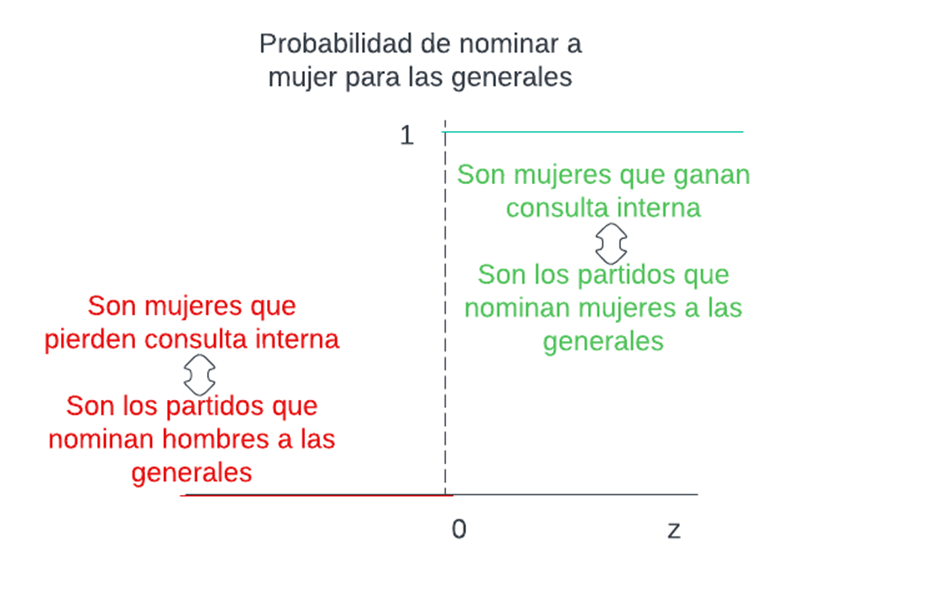
\includegraphics[width=0.8\textwidth]{output/fotocontexto.png}
    \caption{Contextualización ejercicio}
    \label{fig:rdplot}
\end{figure}
Entonces, frente a la pregunta de por qué el cumplimiento de los supuestos permite recuperar el efecto causal en este caso; la respuesta es que los partidos donde las mujeres pierden marginalmente la consulta interna (y por tanto se nomina al hombre) son contrafactuales de los partidos en donde las mujeres ganaron marginalmente (y por tanto se nomina a la mujer).Note que acá, hay que ser cuidadosos con el nivel en el que aplica el supuesto de continuidad de resultados potenciales. No estamos diciendo que hombres justo a la izquierda del umbral son comparables a las mujeres que están justo a la derecha; lo que estamos diciendo es que las mujeres que estaban justo a la izquierda del umbral (las de rojo en la imagen) son comparables con las que están justo a la derecha del umbral (las de verde en la foto). Entonces estos dos grupos van a tener características observables y no observables muy similares. Y esto también incluye a las características de los partidos a los que están asociadas; es decir,los partidos en los que cada una de estas candidatas militan deben ser muy parecidos en cuanto a sus características.\\
Así, si se cumple el supuesto de continuidad local de resultados potenciales, se puede garantizar que no hay cambios bruscos en los resultados esperados a ambos lados del umbral. Además si se cumple el supuesto de no manipulación del cutoff, se puede garantizar que las candidatas no seleccionan estratégicamente su posición relativa al corte y por tanto no tenemos un sesgo de selección. Adicionalmente, perfect complience implica que estamos considerando el efecto total y no toca descontar nada.\\
Si se cumplen estos supuestos, entonces el salto en la función de resultados (el que un partido gane o no la elección general) puede atribuirse exclusivamente al efecto de que el partido haya nominado a una mujer.
\end{solucion}
        \end{enumerate}

\end{enumerate}

Usted cuenta con una base de datos llamada \textit{female\_politics.dta}, que contiene información sobre elecciones primarias y generales en Estados Unidos desde 1972 hasta 2010. Cada observación corresponde a una combinación de candidata, distrito electoral y año. La base de datos permite identificar si la candidata ganó la consulta interna (\textit{primary\_winner} = 1), el margen de victoria o derrota en la lección primaria (\textit{PrimMargin} $> 0$ indica victoria) y si ganó las elecciones generales (\textit{GenWin} = 1). Además, se incluyen algunas características observables.

\begin{enumerate}[resume]
    \item Genere un gráfico\footnote{Recuerde lo visto en la clase complementaria y siga las instrucciones correspondientes.} de la variable de focalización frente a la variable de interés.

    \begin{enumerate}
    
        \item La discontinuidad (o su ausencia) debe ser claramente observable.  
\begin{solucion}
La gráfica se coloca en el literal b) junto con el polinomio de grado 2.
\end{solucion}
        \item Incluya un polinomio global de grado dos en el gráfico. ¿Por qué podría ser preferible un polinomio de grado dos en lugar de uno de mayor grado?
\begin{solucion}
\begin{figure}[H]
    \centering
    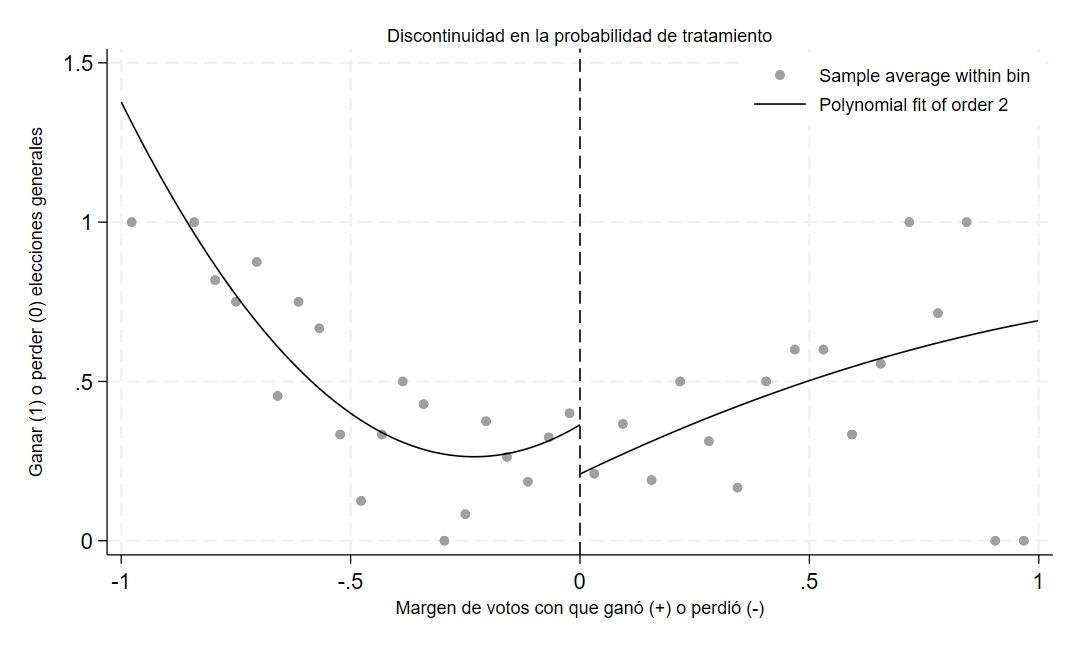
\includegraphics[width=0.8\textwidth]{output/discontinuidad_probabilidad_mean.png}
    \caption{Discontinuidad en la probabilidad de tratamiento}
    \label{fig:rdplot}
\end{figure}
Un polinomio de mayor grado podría causar un overfitting. Esto es que el polinomio empezaría a ajustarse con mucho más detalle a los datos, incluso a pequeñas fluctuaciones aleatorias en los datos,y podría encontrar efectos que en realidad no existen. Esto sería un falso-positivo, entonces uno podría afirmar que es más propenso cometer error tipo 1.\\
En general, overfitting lleva a resultados desacertados y acarrea problemas en la replicabilidad o validez externa del estudio.
\end{solucion}
        \item Interprete los resultados obtenidos. Sea explícito en describir qué sucede en el punto de corte. Intuitivamente, ¿cree que estos resultados tienen sentido? (\textit{máximo 300 palabras}).  
        \begin{solucion}
       La gráfica muestra que cuando una mujer gana la consulta interna por un margen estrecho y es nominada por el partido, entonces estos tienen una menor la probabilidad de ganar las elecciones generales. Así, pareciera que el efecto de interés es negativo.\\
       
Este efecto sería indicativo de un sesgo de género que puede existir en la sociedad. En donde a los partidos que están nominando a hombres les va mejor que a los que están nominando mujeres. Una posible explicación de este sesgo de género puede atribuirse a pre-concepciones o diferencias en cuanto a la manera de hombre y mujeres de hacer política. Cuando las candidatas ganan las primarias con márgenes muy estrechos, no logran consolidar el respaldo total del partido, lo que podría llevar a divisiones internas, menor cohesión y pérdida de apoyo en la campaña general, a su vez pueden tener niveles de ética más elevados y pueden inclinarse por formas más convencionales y aceptables de hacer campaña. Por otro lado, cuando las mujeres pierden, es decir cuando los hombres ganan por margenes muy estrechos, pueden ser más arriesgados en la forma como hacen campaña y en algunas ocasiones poner en riesgo su candidatura.\\ 

Hay muchas teorías detrás y esta es solo una de ellas, pero el punto es que en el caso ideal uno esperaría no encontrar ningún efecto. Sin embargo, la gráfica enciende una preocupación sobre una posible desventaja que tengan las mujeres en el quehacer político e invita a reflexionar sobre las dinámicas internas de los partidos y posibles desigualdades de género en la política electoral
\end{solucion}
    \end{enumerate}

    \item Estime el efecto de que una mujer gane la consulta interna sobre su probabilidad de victoria en las elecciones generales. Para ello, utilice dos enfoques: i) regresión lineal local y ii) polinomio global de grado 2. Para cada enfoque:

    \begin{enumerate}

        \item Explique de manera intuitiva las ventajas y desventajas del método seleccionado (\textit{máximo 150 palabras por propuesta}).
\begin{solucion}
\subsection*{Regresión lineal local}
\textbf{Ventajas }

\begin{itemize}
     \item Ofrece estimaciones más robustas a valores atípicos, ya que ajusta una recta en un entorno local alrededor del punto de corte.
    \item Es menos susceptible a problemas de sobreajuste (\textit{overfitting}) y a error de especificación de la forma funcional en comparación con modelos parametrizados.
    \item Hay campo para pruebas de robustez pues se pueden variar muchas cosas: el ancho de banda, el kernel, etc.
\end{itemize}

\textbf{Desventajas }

\begin{itemize}
    \item La elección del ancho de banda es crucial y puede influir significativamente en las estimaciones; un ancho de banda muy pequeño puede resultar en estimaciones ruidosas, menos muestra y por lo tanto menos precsión, mientras que uno muy grande puede suavizar demasiado las diferencias en los datos

    \item La regresión lineal local puede no captar patrones más complejos en los datos si la relación subyacente no es lineal en la zona cercana al punto de corte.
\end{itemize}


\subsection*{Polinomio global de grado 2}

\textbf{Ventajas}

\begin{itemize}
    \item El uso de un polinomio de grado 2 puede captar mejor las curvaturas en los datos, lo que es útil si la relación entre las variables no es lineal. Esto puede proporcionar un ajuste más adecuado si la verdadera relación tiene una forma más compleja.
    \item Mayor precisión (menor varianza) pues utiliza la totalidad de la muestra
\end{itemize}

\textbf{Desventajas  }

\begin{itemize}
    \item Los polinomios de grado más alto pueden ser susceptibles al sobreajuste (\textit{overfitting}).  
    \item Arriesga no capturar el efecto de tratamiento deseado si se especifica mal la forma funcional 
\end{itemize}

\end{solucion}
        \item Escriba explícitamente la ecuación a estimar.
\begin{solucion}
La ecuación a estimar de manera general es: 
 \begin{equation}\label{ecuacionrd}
Y_i = \alpha  +\tau \cdot D_i \cdot Female_i + f(z)+\varepsilon_i
\end{equation}

\textbf{Regresión lineal local}\\
Usando \ref{ecuacionrd}, en este caso $f(z)$ es un polinomio de grado 1 en $z$, esto es $f(z)=\beta_1 Z_i +\beta_2 (\text{Female}_i \cdot D_i )\cdot Z_i$. El último término lo añadimos porque estamos permitiendo diferentes pendientes a ambos lados del threshold. Entonces la ecuación a estimar sería:

% 
% \begin{equation*}
% Y_i = \alpha + \tau \cdot \text{Female}_i \cdot D_i + \delta_1 Z_i + \beta_1\text{Female}_i + \beta_2 D_i + \varepsilon_i
% \end{equation*}

$$
Y_i = \alpha + \tau \cdot D_i  \cdot \text{Female}_i + \beta_1 Z_i +\beta_2 ( D_i  \cdot \text{Female}_i )\cdot Z_i + \varepsilon_i$$

\vspace{0.5cm}

\textbf{Polinomio global de grado 2}\\
Usando \ref{ecuacionrd}, en este caso $f(z)$ es un polinomio de grado 2 en $z$, esto es $f(z)=\beta_1 Z_i +\beta_2 (\text{Female}_i \cdot D_i )\cdot Z_i +\beta_3 Z_i^2+ \beta_4 (\text{Female}_i \cdot D_i )\cdot Z_i^2 $. La ecuación a estimar sería:

$$
Y_i = \alpha + \tau \cdot D_i  \cdot \text{Female}_i + \beta_1 Z_i +\beta_2 (\text{Female}_i \cdot D_i )\cdot Z_i +\beta_3 Z_i^2+ \beta_4 (\text{Female}_i \cdot D_i )\cdot Z_i^2+ \varepsilon_i$$


En ambos enfoques, \(\tau\) es el parámetro de interés que captura el efecto causal de que una mujer haya ganado marginalmente la consulta interna sobre la probabilidad de que su partido gane la elección general. 
\begin{mdframed}[backgroundcolor=moraditoClaro]
\textbf{Caveat:}A manera de complementar el ejercicio, la especificación se puede hacer con controles; sin embargo en el caso de RD la estimación con y sin controles deberia producir coeficientes muy similares. Los solo servirían para reducir la varianza del modelo y ganar eficiencia. La razón es por la continuidad de resultados potenciales, ya que las mujeres que ganan y las que pierden la consulta interna por margenes muy estrechos son muy parecidas y  no deberían tener características observables significativamente distintas. Aún así: \\

La ecuación a estimar de manera general es
 \begin{equation} 
Y_i = \alpha  +\tau \cdot D_i \cdot Female_i + f(z)+ \gamma \textbf{x}_i+\varepsilon_i
\end{equation}

\textbf{Regresión lineal local}\\
$$
Y_i = \alpha + \tau \cdot D_i  \cdot \text{Female}_i + \beta_1 Z_i +\beta_2 ( D_i  \cdot \text{Female}_i )\cdot Z_i +\gamma \textbf{x}_i+ \varepsilon_i$$

\textbf{Polinomio global de grado 2}
$$
Y_i = \alpha + \tau \cdot D_i  \cdot \text{Female}_i + \beta_1 Z_i +\beta_2 (\text{Female}_i \cdot D_i )\cdot Z_i +\beta_3 Z_i^2+ \beta_4 (\text{Female}_i \cdot D_i )\cdot Z_i^2+\gamma \textbf{x}_i+ \varepsilon_i$$
\end{mdframed}

\end{solucion}
        \item Discuta si es adecuado incluir controles en la regresión. Justifique su decisión (\textit{máximo 150 palabras}).
\begin{solucion}
\textbf{Tanto para el enfoque de regresión lineal local como usando polinomio de grado 2: }
Si se cumplen los supuestos del diseño de regresión discontinua (RD), particularmente la continuidad local de los resultados potenciales, entonces incluir controles no es necesario. Esto se debe a que, cerca del punto de corte, las candidatas a ambos lados deberían ser comparables en promedio, y cualquier salto en el resultado puede atribuirse al hecho de haber sido nominada o no por el partido. Sin embargo, incluir controles puede mejorar la precisión del estimador al reducir la varianza del término de error, aunque no cambia sustancialmente la interpretación causal. En resumen, los controles no son necesarios para la validez del RD, pero pueden ser útiles para ganar eficiencia.
\end{solucion}
        \item Como prueba de robustez, en la regresión lineal local utilice tres anchos de banda: $BW = 0.15, 0.10$ y $0.05$.
\begin{solucion}
Nota: se incluyen los resultados para la estimación parámetrica tanto para los bandwiths como para la muestra total. El último solo se incluye a manera de complementar los resultados, pero no son informativos sobre el efecto pues buscamos es un efecto local y no global. Además, también se incluye la regresión no parámetrica con kernel triangular ya que los resultados con kernel uniforme son los mismos de la regresión parámetrica. La comparativa de los resultados se encuentra en la tabla a continuación. Posteriormente, se va desglosando cada resultado en detalle:

\subsection*{I. Consolidado de resultados}

\begin{table}[H]
\centering
\caption{Regresiones lineales locales de ganar elecciones generales en margen de victoria de primarias}
\resizebox{\linewidth}{!}{%
  
\begin{tabular}{lcccccc}
\hline\hline
 & \multicolumn{3}{c}{Sin controles} & \multicolumn{3}{c}{Con controles} \\
\cline{2-7}
 & BW = .15 & BW = .10 & BW = .05 & BW = .15 & BW = .10 & BW = .05 \\
\hline
Gana Primaria &    -0.249 &    -0.198 &     0.581 &    -0.249 &    -0.198 &     0.581 & \\
 & (    0.344) & (    0.442) & (    0.736) & (    0.344) & (    0.442) & (    0.736) & \\
\hline\hline
\end{tabular}
}
{\footnotesize Nota: Errores estándar en paréntesis.}
\end{table}





    
\subsection*{II. Estimación parámetrica sin controles}
\textbf{Regresión lineal local sin controles}
\begin{table}[H]
\centering
\caption{Estimación paramétrica con regresión local lineal}
\label{tab:interaction_linear}
\begin{tabular}{lcccc}
\toprule
\multicolumn{5}{c}{\textbf{Elecciones Generales}} \\
\cmidrule(lr){2-5}
& Full Sample & BW = 0.05 & BW = 0.1 & BW = 0.15\\
\midrule
Ganar mujer primaria & 0.021 & -0.369$^{**}$ & -0.345 & -0.365 \\
& (0.067) & (0.183) & (0.234) & (0.346) \\
Margen primaria  & -0.627$^{***}$ & 5.056$^{*}$ & 3.784 & 18.939 \\
& (0.108) & (2.786) & (5.620) & (15.668) \\
(Ganar  mujer$\times$ margen) primaria & 1.155$^{***}$ & -2.610 & -1.775 & -32.991 \\
& (0.172) & (4.187) & (8.503) & (21.522) \\
Constant & 0.207$^{***}$ & 0.529$^{***}$ & 0.514$^{***}$ & 0.716$^{***}$ \\
& (0.045) & (0.134) & (0.168) & (0.259) \\
\midrule
Observations & 484 & 98 & 64 & 36 \\
$R^2$ & 0.089 & 0.050 & 0.056 & 0.159 \\
\bottomrule
\end{tabular}
\begin{tablenotes}
\small
\item \textit{Notas:} Errores estándar robustos entre paréntesis. $^{*}p<0.1$, $^{**}p<0.05$, $^{***}p<0.01$.
\end{tablenotes}
\end{table}


\textbf{Polinomio global de grado 2 sin controles}\\
\begin{table}[H]
\centering
\caption{Estimación paramétrica con polinomio de grado 2.}
\label{tab:interaction_quadratic}
\begin{tabular}{lcccc}
\toprule
\multicolumn{5}{c}{\textbf{Elecciones Generales}} \\
\cmidrule(lr){2-5}
& Full Sample & BW = 0.05 & BW = 0.1 & BW = 0.15 \\
\midrule
Ganar mujer primaria & -0.155$^{*}$ & -0.344 & -0.258 & 0.474 \\
& (0.093) & (0.294) & (0.390) & (0.617) \\
Margen primaria & 0.869$^{**}$ & 10.296 & 26.025 & -90.808 \\
& (0.427) & (12.794) & (25.398) & (73.124) \\
(Ganar mujer $\times$ margen) primaria & -0.177 & -15.794 & -59.788$^{*}$ & 11.799 \\
& (0.629) & (18.478) & (35.643) & (93.582) \\
Margen primaria $^2$ & 1.882$^{***}$ & 67.729 & 418.048 & -4011.499$^{*}$ \\
& (0.495) & (156.756) & (459.804) & (2346.737) \\
(Ganar mujer $\times$ margen $^2$) primaria  & -2.092$^{***}$ & 40.525 & 298.913 & 6608.877$^{**}$ \\
& (0.770) & (235.062) & (662.952) & (3028.438) \\
Constant & 0.364$^{***}$ & 0.595$^{***}$ & 0.711$^{**}$ & 0.145 \\
& (0.064) & (0.214) & (0.292) & (0.474) \\
\midrule
Observations & 484 & 98 & 64 & 36 \\
$R^2$ & 0.113 & 0.056 & 0.107 & 0.265 \\
\bottomrule
\end{tabular}
\begin{tablenotes}
\small
\item \textit{Notas:} Errores estándar robustos entre paréntesis. $^{*}p<0.1$, $^{**}p<0.05$, $^{***}p<0.01$.
\end{tablenotes}
\end{table}

 \subsection*{III. Estimación no parámetrica sin controles y Kernel Triangular}
\textbf{Regresión lineal local sin controles}

\begin{table}[H]
\centering
\caption{Efecto de ganar la primaria sobre ganar la elección general (RDD)}
\label{tab:rdd_genwin_bandwidths}
\begin{tabular}{lccc}
\toprule
\multicolumn{4}{c}{\textbf{Elecciones Generales}} \\
\cmidrule(lr){2-4}
& BW = 0.05 & BW = 0.1 & BW = 0.15 \\
\midrule
Ganar mujer primaria & -0.01997 & -0.29981 & -0.35964 \\
Error estándar       & (0.43687) & (0.27632) & (0.21548) \\
\bottomrule
\end{tabular}
\end{table}


\textbf{Polinomio global de grado 2 sin controles}
\textbf{Regresión lineal local sin controles}

\begin{table}[H]
\centering
\caption{Efecto de ganar la primaria sobre ganar la elección general (RDD, polinomio de orden 2)}
\label{tab:rdd_genwin_bandwidths_poly2}
\begin{tabular}{lccc}
\toprule
\multicolumn{4}{c}{\textbf{Elecciones Generales}} \\
\cmidrule(lr){2-4}
& BW = 0.05 & BW = 0.1 & BW = 0.15 \\
\midrule
Ganar mujer primaria & 0.58144  & -0.19762 & -0.24940 \\
Error estándar       & (0.73556) & (0.44238) & (0.34408) \\
\bottomrule
\end{tabular}
\end{table}

\subsection*{IV. Estimación parámetrica con controles}
Se presenta igualmente la regresión con controles (los usados en el paper original): \textit{
 Presidential Vote Share en T-1, Dummy de Incumbent, Presidential Election Year, y
Decade
 }. No obstante, idealmente se deberían llegar a coeficientes similares tanto como con como sin controles, por la argumentación del literal c). \\
 
\textbf{Regresión lineal local con controles}

\begin{table}[H]\centering
\caption{Efecto de ganar la primaria sobre el resultado en la elección general (con controles)}
\label{tab:rd_controls_full}
\footnotesize
\begin{tabular}{lcccc}
\toprule
 \multicolumn{5}{c}{\textbf{Elecciones Generales}} \\
\cmidrule(lr){2-5}
& Full Sample & BW = 0.05 & BW = 0.1 & BW = 0.15 \\
\midrule
\textbf{Ganó primaria} & 0.001 & -0.482$^{**}$ & -0.422$^{**}$ & -0.339$^{**}$ \\
 & (0.054) & (0.227) & (0.181) & (0.153) \\
\textbf{Margen primaria} & -0.468$^{***}$ & 25.190$^{**}$ & 3.015 & 3.727 \\
 & (0.096) & (10.294) & (4.377) & (2.525) \\
\textbf{Ganó primaria $\times$ Margen} & 0.370$^{***}$ & -34.130$^{**}$ & 1.005 & -1.827 \\
 & (0.132) & (14.828) & (6.606) & (3.663) \\
\midrule
\textbf{Controles} \\
Presidencial & 0.018$^{***}$ & 0.018$^{***}$ & 0.019$^{***}$ & 0.018$^{***}$ \\
 & (0.002) & (0.006) & (0.004) & (0.004) \\
Año presidencial & -0.071$^{**}$ & -0.127 & -0.176 & -0.083 \\
 & (0.034) & (0.128) & (0.105) & (0.079) \\
Titular (inc) & 0.604$^{***}$ & -- & 0.774$^{***}$ & 0.604$^{***}$ \\
 & (0.046) & (omitido) & (0.156) & (0.145) \\
Periodo 1982--1990 & -0.028 & -0.176 & -0.204 & 0.047 \\
 & (0.063) & (0.292) & (0.192) & (0.131) \\
Periodo 1992--2000 & 0.265$^{***}$ & -0.126 & 0.073 & 0.152 \\
 & (0.058) & (0.214) & (0.142) & (0.125) \\
Periodo 2002--2010 & 0.224$^{***}$ & 0.205 & 0.150 & 0.284$^{**}$ \\
 & (0.058) & (0.211) & (0.147) & (0.132) \\
\midrule
Constante & -0.779$^{***}$ & -0.153 & -0.443 & -0.568$^{*}$ \\
 & (0.090) & (0.496) & (0.360) & (0.299) \\
\midrule
Observaciones & 484 & 36 & 64 & 98 \\
R$^2$ & 0.466 & 0.548 & 0.444 & 0.371 \\
\bottomrule
\multicolumn{5}{p{13cm}}{\footnotesize Nota: Errores estándar robustos entre paréntesis. * p$<$0.10, ** p$<$0.05, *** p$<$0.01. La variable \textit{inc} se omite en la muestra estrecha de $\pm$0.025 por colinealidad.}
\end{tabular}
\end{table}



\textbf{Polinomio global de grado 2 con controles}\\
\begin{table}[H]\centering
\caption{Efecto de ganar la primaria sobre el resultado en la elección general (con controles)}
\label{tab:rd_controls_full}
\footnotesize
\begin{tabular}{lcccc}
\toprule
\multicolumn{5}{c}{\textbf{Elecciones Generales}} \\
\cmidrule(lr){2-5}
& Full Sample & BW = 0.05 & BW = 0.1 & BW = 0.15  \\
\midrule
\textbf{Ganó primaria} & -0.166$^{**}$ & 0.197 & -0.433$^{*}$ & -0.352 \\
 & (0.075) & (0.270) & (0.253) & (0.219) \\
\textbf{Margen primaria} & 0.554 & -59.836 & 22.383 & 9.598 \\
 & (0.354) & (38.040) & (17.550) & (9.577) \\
\textbf{Ganó primaria $\times$ Margen} & -0.125 & -6.022 & -36.565 & -13.305 \\
 & (0.489) & (55.566) & (27.746) & (14.769) \\
\textbf{Margen primaria$^2$} & 1.292$^{***}$ & -3109.127$^{**}$ & 367.132 & 75.413 \\
 & (0.419) & (1365.350) & (352.618) & (124.533) \\
\textbf{Ganó primaria $\times$ Margen$^2$} & -1.976$^{***}$ & 5392.971$^{**}$ & 7.433 & 0.599 \\
 & (0.573) & (1954.299) & (535.979) & (191.072) \\
\midrule
\textbf{Controles} \\
Presidencial & 0.018$^{***}$ & 0.017$^{**}$ & 0.018$^{***}$ & 0.018$^{***}$ \\
 & (0.002) & (0.006) & (0.005) & (0.004) \\
Año presidencial & -0.072$^{**}$ & -0.104 & -0.166 & -0.077 \\
 & (0.034) & (0.124) & (0.105) & (0.079) \\
Titular (inc) & 0.616$^{***}$ & -- & 0.713$^{***}$ & 0.630$^{***}$ \\
 & (0.046) & (omitido) & (0.166) & (0.151) \\
Periodo 1982--1990 & -0.027 & -0.165 & -0.182 & 0.042 \\
 & (0.062) & (0.307) & (0.189) & (0.133) \\
Periodo 1992--2000 & 0.270$^{***}$ & -0.057 & 0.039 & 0.148 \\
 & (0.057) & (0.232) & (0.152) & (0.128) \\
Periodo 2002--2010 & 0.212$^{***}$ & 0.256 & 0.173 & 0.273$^{**}$ \\
 & (0.057) & (0.224) & (0.153) & (0.135) \\
\midrule
Constante & -0.648$^{***}$ & -0.610 & -0.245 & -0.484 \\
 & (0.106) & (0.494) & (0.370) & (0.333) \\
\midrule
Observaciones & 484 & 36 & 64 & 98 \\
R$^2$ & 0.480 & 0.611 & 0.462 & 0.376 \\
\bottomrule
\multicolumn{5}{p{13cm}}{\footnotesize Nota: Errores estándar robustos entre paréntesis. * p$<$0.10, ** p$<$0.05, *** p$<$0.01. La variable \textit{inc} se omite en la muestra estrecha de $\pm$0.025 por colinealidad.}
\end{tabular}
\end{table}



\end{solucion}
        \item Interprete los resultados obtenidos. ¿Qué conclusiones se pueden extraer de este análisis? (\textit{máximo 200 palabras}).
\begin{solucion}
En ambos modelos se observa que, cuando una mujer gana la elección primaria con un margen estrecho y es nominada, la probabilidad de que su partido gane la elección general disminuye. Este patrón se mantiene al variar el \textit{bandwidth}, y la magnitud del efecto es bastante similar entre especificaciones. En el caso de la regresión local lineal, con un \textit{bandwidth} de 0.15, ganar la primaria reduce en 37 puntos porcentuales la probabilidad de éxito en la general, un efecto que es estadísticamente significativo al 5\%. Aunque al reducir el \textit{bandwidth} el efecto pierde significancia, su dirección se mantiene y las fluctuaciones en magnitud no son extremas. \\

Por otro lado, la especificación con un polinomio de grado 2 arroja resultados comparables en términos de magnitud. Se incluyen los coeficientes de la muestra completa como referencia, aunque es importante resaltar que las estimaciones de interés deben centrarse en el entorno cercano al umbral, donde el margen de victoria o derrota tiende a cero. \\

Estos resultados sugieren posibles divisiones dentro de los partidos que se agudizan cuando las mujeres ganan por márgenes estrechos. Esto podría indicar la presencia de sesgo de géneros, en donde se agudiza la falta de apoyo y de cohesión interna dentro del partido.



\end{solucion}
    \end{enumerate}
    \item En su investigación, \href{https://link.springer.com/article/10.1007/s11109-017-9407-7}{Bucchianeri (2018)} es muy cuidadoso con la interpretación del efecto estimado: ``[...] es importante aclarar que el diseño de regresión discontinua (RDD) en este caso está identificando el efecto causal de nominar a una candidata [mujer] y no el efecto causal del género.'' 

    \begin{enumerate}
        \item ¿Cuál es la diferencia entre los dos efectos que el autor menciona?
\begin{solucion}
Note que ambos efectos son muy distintos. Específicamente:

\begin{itemize}
    \item \textbf{Efecto causal de nominar a una candidata (mujer):} en este estamos suponiendo que las mujeres que ganan  y que pierden por un margen muy estrecho la consulta interna, son comparables. El efecto de interés es recuperable de manera local ya que cualquier salto en la probabilidad de ganar en las elecciones puede atribuirse exclusivamente al hecho de haber nominado o no una candidata mujer. Ahora, note que este efecto incopora el efecto de género, más otras cosas. Las candidatas que ganan por poco margen en las primarias son, en promedio, similares a aquellas que las pierden por poco. Como resultado, el efecto causal estimado a partir del diseño de regresión discontinua es una combinación del efecto de nominar a una candidata mujer y del efecto de las características asociadas al género. Entonces acá el efecto esta incorporando todo los asociado al género que acompañan dicha nominación, incluidos tanto los posibles desventajas que enfrentan las mujeres como las ventajas que pueden aprovechar durante sus campañas.Por ejemplo,  si las mujeres nominadas por margen estrecho tiene mayor educación que los hombres que pierden marginalmente, entonces el efecto estimado representará el efecto total de nominar estrechamente a una candidata femenina de calidad ligeramente superior en lugar de un candidato masculino de calidad ligeramente inferior, y esto ya tiene en cuenta todos los demás aspectos que pueden varíar con el género.
    
    
    \item \textbf{Efecto causal del género:} este consideraría el efecto de ser hombre o mujer en la probabilidad de ganar las elecciones generales. Para  estimar el efecto localmente con el RD, entonces ahora el tratamiento se define como ser o no mujer dado que se ganó la elección cerrada. Entonces tocaría decir que la muestra de hombres y mujeres que ganan marginalmente la consulta interna es, en promedio, similar en características subyacentes. En otras palabras, que sus característica observables y no observables van a ser estadísticamente iguales. Pero esto es una afirmación muy fuerte, pues hay características que varían fácilmente por género, por ejemplo el estilo de comunicación, forma de hacer política, la edad también podría ser sistemáticamente diferente, etc. Así, el género podría no ser el único atributo que varía entre los hombres y las mujeres que ganan por un margen estrecho la consulta interna, apareciendo así un problema de comparabilidad.  Por ejemplo, 
   Por tanto, el diseño del RD planteado no sería la mejor estrategia para identificar el efecto causal del género sobre la probabilidad de ganar las elecciones generales, en este contexto.
\end{itemize}
\end{solucion}
        \item ¿Por qué cree usted que el autor descarta la segunda interpretación?
\begin{solucion}
El problema es que hay muchas variables más allá del género que pueden estar cambiando entre los hombres y las mujeres que ganan las elecciones primarias. Entonces no hay continuidad de resultados potenciales y los grupos no serían comparables. Por tanto, el diseño de RD podría complicar las cosas ya que no está aislando el género como única fuente de variación. Si el autor quisiese encontrar el efecto causal del género, el problema se complejiza y debería re-plantear el diseño, pero también tendría que re-evaluar sus datos, el contexto, etc. Esta es la razón por la que creo que el autor decide elegir la primera interpretación. Usando esta, puede proveer una argumentación más consistente y sus resultados son más creíbles.
\end{solucion}
        \item Si usted fuera la investigadora, ¿qué efecto consideraría más deseable recuperar? Sustente teniendo en cuenta la \textbf{validez} del diseño experimental y los obstáculos para la identificación.
\begin{solucion}
Consideraría más deseable recuperar el primer efecto. Este es más creible, ya que tiene en cuenta que puede haber diferencias entre hombres y mujeres que ganan la consulta interna.\\

El efecto de nominar a una candidata mujer ya incorpora todas las características asociadas al género que acompañan la nominación, entonces es un efecto que ya abarca las diferencias sistemáticas entre hombres y mujeres. Por ejemplo, si ocurriese que las mujeres nominadas en las primarias, en promedio, cuentan con mayor educación o experiencia que los hombres nominados, entonces el efecto que se computa con el RD representa el efecto total de nominar a una mujer ligeramente de mayor calidad en lugar de a un hombre ligeramente de menor calidad.\\

Como ya mencioné arriba, un efecto causal de solo género tendría menor validez interna, no es del todo recuperable  con este diseño de RD, de \textit{close election } especificamente, pues otras variables estarían cambiando y la discontinudad en la probabilidad de ganar las generales no va a ser solo atribuible a ser hombre o mujer ( note que no ocurre en el ejemplo de arriba, la educación también cambia con el genéro).Habría muchos más obstaculos para la identificación, no se cumple resultados potenciales por lo mismo.  Así, tocaría rediseñar el experimento y ver si la estructura de los datos es compatible con el re-diseño, etc. Por tanto, ante todos los problema que supone el segundo efecto en este contexto, preferiría explorar el primer efecto.

% \textcolor{red}{revisar: pg 12 buchaneri, }
\end{solucion}        
    \end{enumerate}
  
    
\end{enumerate}

\bigskip
    
\href{https://onlinelibrary-wiley-com.ezproxy.uniandes.edu.co/doi/full/10.1111/ajps.12741}{Marshall (2024)} argumenta que, aunque estimar efectos causales de una \textbf{característica} de un candidato ganador es deseable, no es evidente que un RD pueda aislar dicho efecto usando el método de \textit{close election}. En particular, argumenta que un RD identifica efectos compuestos de muchas características en lugar de un efecto LATE asociado exclusivamente a la característica de interés. \\

En este sentido, mientras un RD tradicional define el tratamiento como caer arriba o abajo del punto de corte, el RD que estamos estudiando en este ejercicio define el tratamiento como tener vs no tener una característica de interés específica (e.g. ser mujer) \textbf{dado} que dicho político ganó una elección cerrada.\footnote{Esto implica que en este tipo de RDs se están comparando políticos que estuvieron en una elección cerrada, pero que difieren en una característica observada dicótoma (e.g. ser mujer).} Frente a esto, el autor señala dos obstáculos importantes: i) las elecciones cerradas no asignan aleatoriamente (ni \textit{as-good-as-random}) la característica de interés y ii) al concentrarse en elecciones cerradas, la característica de interés puede directamente determinar la variable de focalización (el margen de votos). \\

De ahora en adelante, suponga que se desea responder la pregunta: \textbf{¿cuál es el efecto de ser mujer sobre la probabilidad de obtener la victoria en las elecciones generales?}. El objetivo de los siguientes incisos es identificar las principales dificultades para responder este tipo de preguntas en el contexto de los RD.

\bigskip

\begin{enumerate}[resume]
    
\item Explique intuitivamente ambos obstáculos mencionados por \href{https://onlinelibrary-wiley-com.ezproxy.uniandes.edu.co/doi/full/10.1111/ajps.12741}{Marshall (2024)} usando \textbf{explícitamente} el contexto del caso-estudio de \href{https://link.springer.com/article/10.1007/s11109-017-9407-7}{Bucchianeri (2018)}. Mencione por qué atentan contra la identificación del efecto causal. 

%\item Si las mujeres que ganan elecciones cerradas son sistemáticamente distintas a hombres que ganan elecciones cerradas\footnote{Lo son. Por ejemplo, vea \href{https://onlinelibrary.wiley.com/doi/abs/10.1111/j.1540-5907.2011.00512.x}{Anzia \& Berry (2011)} y \href{https://www.cambridge.org/core/journals/politics-and-gender/article/abs/what-it-takes-to-win-questioning-gender-neutral-outcomes-in-us-house-elections/83267D037A804CE682D5A640DA7B27E0}{Pearson \& McGhee (2011)}}, ¿cree usted que esto puede comprometer el efecto que se desea rescatar?
        \begin{solucion}
\textbf{i)las elecciones cerradas no asignan aleatoriamente (ni as-good-as-random) la
característica de interés}\\
Intuitivamente, esto quiere decir que la probabilidad de ser mujer dado que ganó la nominación es distinta de la probabilidad de ser hombre dado que ganó la nominación
\[
    \mathbb{P}(\text{Mujer} \mid \text{Nominado}) \neq \mathbb{P}(\text{Hombre} \mid \text{Nominado})
    \]

Así, la intuicion es que las mujeres nominadas son sistemáticamente distinta de los hombres nominados. En en contexto de \textit{close elections} que plantea Bucchianeri (2018), no se asigna aleatoriamente la característica de ser mujer, lo que significa que las candidatas femeninas no están en igualdad de condiciones con sus contrapartes masculinas. La naturaleza competitiva de estas elecciones puede llevar a que las mujeres enfrenten barreras adicionales y sesgos basados en género que afectan sus posibilidades de éxito. Esto complica la evaluación del efecto del género en los resultados electorales, ya que la selección de candidatos puede depender de factores que no son distribuidos de manera aleatoria, lo que limita la capacidad de hacer inferencias causales claras sobre el impacto del género en estas situaciones.

\textbf{ii) al concentrarse en elecciones cerradas, la característica de interés puede directamente
determinar la variable de focalización (el margen de votos).}\\
ser hombre o ser mujer puede incidir en los votos que se obtienen al interior del partido, entonces alguien podria preferir votar por la candidata de mujer solo por el hecho de ser mujer, o por el hombre solo por el hecho de ser hombre. En este escenario, como el tratamiento es ser mujer, uno podria argumentar que cuando la competencia esta muy reñida entre el hombre y la mujer, hay gente que simplemente votaria por el hombre, por motivos tradicionales, etc. En palabras, esto es que la probabilidad de ser nominada dado que se es mujer podría ser menor de la probabilidad de ser nominado dado que se es hombre.  \[
    \mathbb{P}(\text{Nominado} \mid \text{Mujer}) < \mathbb{P}(\text{Nominado} \mid \text{Hombre})
    \]

En un escenario competitivo ideal, estas probabilidades deberían ser iguales, pues no debería haber sesgos o estereotipos que afectasen la percepción de los votantes sobre las candidatas.  El margen de votos no debería estar determinada por el hecho de ser mujer o no.\\ 


\textbf{Retos identificación efecto causal}
 Evaluar el efecto de ser mujer sobre la probabilidad de ganar elecciones generales presenta varios retos en la identificación del efecto causal. Primero, los problemas de selección pueden surgir si las mujeres que son nominadas  no son comparables a los de los hombres, confundiendo así el impacto del género con otros factores como la calidad del candidato y el contexto político. Además, la omisión de variables clave como el apoyo del partido y el gasto de campaña puede sesgar las estimaciones. Las percepciones de los votantes y los estereotipos de género influyen en las decisiones electorales, complicando aún más la interpretación de los resultados. Asimismo, la naturaleza competitiva de las elecciones afecta cómo se manifiestan estos efectos, y los hallazgos derivados de clásicos diseños de estudio pueden carecer de generalizabilidad a otros contextos electorales. Estos factores resaltan la necesidad de enfoques de investigación robustos que minimicen sesgos y permitan una identificación clara del impacto del género en el éxito electoral.
 
% \textcolor{red}{revisar!!!!!}      
\end{solucion}
\end{enumerate}

\bigskip

Las preocupaciones de \href{https://onlinelibrary-wiley-com.ezproxy.uniandes.edu.co/doi/full/10.1111/ajps.12741}{Marshall (2024)} pueden implicar un sesgo por un concepto que él llama \textbf{compensadores diferenciales} (\textit{compensating differentials}). Estos se definen como características observadas y/o no-observadas que: 1) son distintas a la característica de interés, y 2) permiten que aunque dos políticos no tengan la misma característica de interés, igualmente se enfrenten en una elección cerrada. \\

Por ejemplo, considere los años de educación de un político. Suponga que los votantes, en igualdad de condiciones, tienen una preferencia general por votar por un hombre en lugar de una mujer, pero a su vez prefieren candidatos con mayor educación. En este caso, la variable de años de educación es un \textbf{compensador diferencial} porque: 1) las variables de años de educación vs ser mujer son teóricamente distintas, y 2) en elecciones cerradas, los hombres van a tener en promedio menos años de educación que las mujeres\footnote{Es decir, los años de educación adicionales que tiene la candidata mujer \textbf{compensa} la desventaja de ser mujer lo suficiente para generar una elección cerrada.}. Note que esto \textbf{no} implica que la variable \textit{años de educación} esté desbalanceada a \textbf{nivel de distrito electoral}. Más bien, indica que, a \textbf{nivel de candidato}, las mujeres que ganan elecciones cerradas difieren de los hombres que también las ganan, más allá de la diferencia de sexo.  \\

En los siguientes incisos, usted va a demostrar que esto implica un sesgo, incluso cuando no hay correlación entre ser mujer y el compensador diferencial. Suponga que ser mujer ($Female_i = 1$) es perjudicial para la probabilidad de ganar una elección general y sea $W_i$ un compensador diferencial que tiene un impacto negativo en la probabilidad de ganar las elecciones generales. \\

Suponga que en una consulta interna fija con dos candidatxs $i$ y $j$, se tiene que:
\vspace{0.2cm}
\begin{equation}\label{votoscandidatoscompensador}
    Votos_i = \beta_F\frac{Female_i-Female_j}{2}+\beta_W\frac{W_i-W_j}{2}+\frac{\epsilon_i-\epsilon_j}{2}
\end{equation}
\vspace{0.2cm}
donde $W_i-W_j \sim \mathcal{N}(0, \sigma_W^2)$ es la resta del compensador diferencial y $\epsilon_i-\epsilon_j \sim \mathcal{N}( 0, \sigma_\epsilon^2)$ es un choque aleatorio. Sea $Y_i^1 = \tau Female_i + \gamma W_i + u_i$ el resultado potencial de que la persona $i$ gane la elección general, con $u_i$ un término de error independiente de todas las variables.

\bigskip

\begin{enumerate}[resume]
    \item Suponga que $Female_i \; \perp\!\!\!\perp \; W_i, W_j$ y que $\tau,\gamma \leq 0$. Demuestre que el estimador de RD está asintóticamente sesgado. Para ello:

    \begin{enumerate}

        \item Explique breve e intuitivamente por qué $Female_i \; \indep \; W_i, W_j$ es un ``best case scenario''.
       \begin{solucion}
La condición $Female_i \; \indep \; W_i, W_j$ implica que el hecho de que una candidata sea mujer no está correlacionada con la característica que es compensadora diferencial de sí misma ni con la de su contrincante. Es decir, el género está asignado de forma casi aleatoria respecto a los atributos que también afectan el resultado electoral. Por ejemplo, si el compensador es poca experiencia en el sector público, entonces ser mujer no está correlacionado con tener menos experiencia ni con que su contrincante tenga menos experiencia, asemejandose a una 'aleatorización'. (Nota: como $W_i$ tiene un efecto negativo, entonces tiene que ser que para los hombres la característica sea alta y para las mujeres la característica sea baja, luego en vez de decir años de educación o años de experiencia en sector publico, se dice años sin educación o poca experiencia en sector público.La interpretación hubiese sido más directa si $W_i$ tuviese impacto positivo)\\

Esto constituye un ``best case scenario'' porque permite interpretar el parámetro $\tau$ como el efecto causal de que la candidata sea mujer, sin que ese efecto esté contaminado por diferencias sistemáticas en otras características relevantes. En otras palabras, elimina el riesgo de confundir el efecto de género con el efecto de variables asociadas al género (como la experiencia en el sector público). Por tanto, cualquier efecto estimado puede ser atribuido directamente a la variable de interés: el género del candidato. 
% \textcolor{red}{revisar}
\end{solucion}
            
        \item Demuestre que si en una consulta interna que enfrenta a una política $i$ y a un político $j$ ambos reciben exactamente el mismo número de votos, entonces

        \begin{equation*}
            \beta_F + \beta_W(W_i - W_j) + (\epsilon_i - \epsilon_j)  = 0.
        \end{equation*}

        Interprete brevemente los mecanismos que podrían justificar este empate.
\begin{solucion}
% \textcolor{red}{Gus}
\textbf{Claim:}$ \beta_F + \beta_W(W_i - W_j) + (\epsilon_i - \epsilon_j)  = 0$
\begin{proof}
Suponga que en una consulta interna que enfrenta a una política $i$ y a un político $j$ ambos reciben exactamente el mismo número de votos. Esto es:
\begin{equation*}
    Votos_i = Votos_j
\end{equation*}

Ahora, sabemos que $Votos_i = \beta_F\frac{Female_i-Female_j}{2}+\beta_W\frac{W_i-W_j}{2}+\frac{\epsilon_i-\epsilon_j}{2}$
    por la ecuación \ref{votoscandidatoscompensador}.  Usando que $Female_i=1, Female_j=0$, entonces:
\begin{equation*}
    Votos_i = \beta_F \cdot \frac{1}{2} + \beta_W \cdot \frac{W_i-W_j}{2}+ \frac{\epsilon_i - \epsilon_j}{2} 
    \end{equation*}
    \begin{equation*}
 Votos_j = \beta_F \cdot \frac{-1}{2} + \beta_W \cdot \frac{W_j-W_i}{2} + \frac{\epsilon_j - \epsilon_i}{2}
\end{equation*}

Entonces
\begin{align*}
    0 &= Votos_i - Votos_j \\
    &= \beta_F \cdot \frac{1}{2} + \beta_W \cdot \frac{W_i - W_j}{2} + \frac{\epsilon_i - \epsilon_j}{2} 
    \quad - \left( \beta_F \cdot \frac{-1}{2} + \beta_W \cdot \frac{W_j - W_i}{2} + \frac{\epsilon_j - \epsilon_i}{2} \right) \\
    &= \beta_F \cdot \frac{1}{2} + \beta_W \cdot \frac{W_i - W_j}{2} + \frac{\epsilon_i - \epsilon_j}{2} + \beta_F \cdot \frac{1}{2} - \beta_W \cdot \frac{W_j - W_i}{2} - \frac{\epsilon_j - \epsilon_i}{2} \\
    &= \beta_F \cdot \left( \frac{1}{2} + \frac{1}{2} \right) + \beta_W \cdot \left( \frac{W_i - W_j}{2} - \frac{W_j - W_i}{2} \right) + \left( \frac{\epsilon_i - \epsilon_j}{2} - \frac{\epsilon_j - \epsilon_i}{2} \right) \\
    &= \beta_F \cdot \left( \frac{2}{2} \right) + \beta_W \cdot \left( 2 \frac{W_i - W_j}{2}  \right) + \left( 2\frac{\epsilon_i - \epsilon_j}{2} \right) \\
    &= \beta_F + \beta_W(W_i - W_j) + (\epsilon_i - \epsilon_j) 
\end{align*}
Por tanto:
\begin{align*}
  \beta_F + \beta_W(W_i - W_j) + (\epsilon_i - \epsilon_j) &= 0
\end{align*}
\end{proof}
\textbf{Interpretación:} Si una mujer y un hombre empatan en una elección primaria, el efecto negativo asociado a ser mujer ($\beta_F < 0$) debe estar siendo compensado por una combinación de mejores características observables \(\beta_W(W_i - W_j) > 0 \).  Específicamente, esta diferencia puede  atribuirse a que las candidatas tengan mayores niveles de educación o años de experiencia en el sector público respecto a los hombres; esto se refleja en $W_i < W_j$, y se traduce en una contribución positiva al diferencial de votos pues $\beta_W < 0$. \\ %Por su parte, la segunda diferencia $\epsilon_i - \epsilon_j$ puede atribuirse a factores no observables capturados en el término de error, como el que las mujeres tengan mayores habilidades interpersonales, capacidad de movilización, carisma o redes dentro del partido, etc \\

En conjunto, esta condición sugiere que las mujeres que logran empatar con hombres en elecciones internas deben superar la desventaja inicial de ser discriminadas por su género, mediante mayores credenciales o ventajas de sus características (como experiencia, carisma, educación, o redes políticas) .


\end{solucion}
        \item Demuestre que $\plim_{n \to \infty} \mid\hat{\tau}_{RD} \mid< \mid\tau\mid$. 
        \begin{solucion}
\textbf{Claim:}$\plim_{n \to \infty} \mid \hat{\tau}_{RD}\mid < \mid \tau\mid$
\begin{proof}
Dado que estamos interesados en el caso en que el margen en la primaria es cercano a cero, tomamos \( z_0 = 0 \). Además, como sólo uno de los dos gana la primaria, consideramos la diferencia de resultados si ambos hubieran pasado a la elección general. Luego:
\[
\tau_{RD} := \mathbb{E}[Y_i^{1} - Y_j^{1} \mid z = 0]
\]

Usamos la función de resultado potencial:
\[
Y_i^{1} = \tau \cdot Female_i + \gamma W_i + u_i
\]

Reemplazando:
\begin{align*}
\tau_{RD} 
&= \mathbb{E}\left[\left(\tau \cdot Female_i + \gamma W_i + u_i\right) - \left(\tau \cdot Female_j + \gamma W_j + u_j\right) \mid Female_i = 1, Female_j = 0, z = 0\right] \\
&= \mathbb{E}\left[\tau + \gamma (W_i - W_j) + (u_i - u_j) \mid Female_i = 1, Female_j = 0, z = 0\right] 
\end{align*}
Aplicando linealidad y propiedades del valor esperado: 
\begin{align*}
 \tau_{RD} &=\tau + \gamma \cdot \mathbb{E}[W_i - W_j \mid Female_i = 1, Female_j = 0, z = 0] \nonumber\\
 & + \mathbb{E}[u_i - u_j \mid Female_i = 1, Female_j = 0, z = 0]
\end{align*}
Como \( u_i \) es independiente de \( z \), \( W_i \), \( W_j \), y \( Female \), se cumple que:
\[
\mathbb{E}[u_i - u_j \mid z = 0, Female_i = 1, Female_j = 0] = 0
\]
Además, note que por el supuesto de $Female_i \; \perp\!\!\!\perp \; W_i, W_j$ tenemos que $\mathbb{E}[W_i - W_j \mid Female_i = 1, Female_j = 0, z = 0] =  \mathbb{E}[W_i - W_j \mid z = 0]$. Luego:
\begin{align}\label{deftauRD}
\tau^{RD} =\tau + \gamma \cdot \mathbb{E}[W_i - W_j \mid  z = 0]
\end{align}

Ahora, dado que \( W_i - W_j \) y \( \varepsilon_i - \varepsilon_j \) son normales e independientes, y \( z= \beta_F + \beta_W(W_i - W_j) + (\epsilon_i - \epsilon_j) \) es una combinación lineal de ellos, también es normal. Por lo tanto, la esperanza condicional se puede escribir usando la fórmula de la esperanza condicional en normales conjuntas:
\[
\mathbb{E}[W_i - W_j \mid z = 0] = \frac{\text{Cov}(W_i - W_j, z)}{\text{Var}(z)} (0 - \mathbb{E}[z])
\]
La intuición de esta prueba se muestra \hyperlink{claimesperanzacondicional}{acá abajo} \\
Usando el análogo muestral de \ref{deftauRD}, aplicando el p-lim y sus propiedades, tenemos:
\begin{align*}
\plim_{n \to \infty} \hat{\tau}_{RD} 
&=  \tau + \gamma \cdot \frac{\text{Cov}(W_i - W_j, z)}{\text{Var}(z)} \cdot (-\mathbb{E}[z])
\end{align*}
Ahora, para obtener cada uno de los valores tenemos:\\
\textbf{Cálculo de  \(\mathbb{E}[z]\):}
\[
\mathbb{E}[z] = \beta_F + \beta_W \mathbb{E}[ W_i - W_j] + \mathbb{E}[\varepsilon_i - \varepsilon_j] = \beta_F + 0 + 0 = \beta_F
\]

\textbf{Cálculo de \(\text{Cov}( W_i - W_j, z)\):}
\begin{align*}
\text{Cov}( W_i - W_j, z)  &= \text{Cov}( W_i - W_j, \beta_W ( W_i - W_j) + (\varepsilon_i - \varepsilon_j)) \\
&= \beta_W  \text{Var}( W_i - W_j) + \text{Cov}
 (  W_i  , \varepsilon_i-\varepsilon_j) -\text{Cov}
 (  W_j , \varepsilon_i-\varepsilon_j) \\
 &= \beta_W \cdot \text{Var}( W_i - W_j)   \quad \text{(Como $ \varepsilon_i-\varepsilon_i$ es choque aleatorio)}\\ 
 &= \beta_W \sigma_W^2 \quad \text{(Como $\text{Var}( W_i - W_j)=\sigma_W^2$)}
\end{align*}

 

\textbf{Cálculo de \(\text{Var}(z)\):}
\begin{align*}
\text{Var}(z) &= \text{Var}(\beta_W ( W_i - W_j) + (\varepsilon_i - \varepsilon_j))\\
& =  \beta_W \text{Var}( W_i - W_j) + \text{Var}(\varepsilon_i - \varepsilon_j)+ 2\beta_W  \text{Cov}(W_i - W_j, \varepsilon_i - \varepsilon_j) \\
& =  \beta_W \text{Var}( W_i - W_j) + \text{Var}(\varepsilon_i - \varepsilon_j) \quad \text{(Como $ \varepsilon_i-\varepsilon_i$ es choque aleatorio)}\\
& = \beta_W^2 \sigma_W^2 + \sigma_\varepsilon^2
\end{align*}


Reemplazando estos valores, entonces:
\begin{align*}
\plim_{n \to \infty} \mid\hat{\tau}_{RD}\mid  = \mid\tau \mid-\gamma \cdot \frac{\beta_W \sigma_W^2}{\beta_W^2 \sigma_W^2 + \sigma_\varepsilon^2} (\beta_F)
\end{align*}

Sabemos que $\beta_F,  \beta_W ,\gamma< 0$ entonces el sesgo $- \gamma \cdot \frac{\beta_W \sigma_W^2}{\beta_W^2 \sigma_W^2 + \sigma_\varepsilon^2} (\beta_F)$ es positivo, y se concluye que:
\[
\plim_{n \to \infty} \mid\hat{\tau}_{RD}\mid < \mid\tau\mid
\]
\end{proof}



 \begin{mdframed}[backgroundcolor=moraditoClaro]
\hypertarget{claimesperanzacondicional}{}
      \textbf{Claim:} Sea  \( W_i - W_j \) y \( \varepsilon_i - \varepsilon_j \)  variables normales e independientes, y \( z = \) una combinación lineal de ellos. Entonces, la esperanza condicional $$\mathbb{E}[W_i - W_j \mid z = 0] = \frac{\text{Cov}(W_i - W_j, z)}{\text{Var}(z)} (0 - \mathbb{E}[z])$$\\
    
      \begin{proof}
    Sabemos que \( \varepsilon_i - \varepsilon_j \sim \mathcal{N}(0, \sigma_\varepsilon^2) \), y \(  W_i - W_j \sim \mathcal{N}(0, \sigma_W^2) \), además independientes.

Además, sabemos que \( z \) está definido como:
\[
z = \beta_F + \beta_W(W_i - W_j) + (\varepsilon_i - \varepsilon_j)
\]

Luego $z$ es una combinación de normales, luego es normal también. Y en particular $E[z]=0$.

Luego, dado que \(  W_i - W_j \) y \( z \) son combinaciones lineales de normales, su distribución conjunta es normal.Ahora, la esperanza condicional de $W_i - W_j$ es lineal en \( z \). Es decir, existe una relación de la forma:

\[
\mathbb{E}[W_i - W_j  \mid z = z_0] = a + b z_0
\]

El problema es encontrar constantes \( a \) y \( b \) tal que esta ecuación se cumpla. Sabemos, por resultado del modelo de regresión lineal, que el mejor predictor lineal de \( W_i - W_j  \) dado \( z \) está dado por:

\[
\mathbb{E}[W_i - W_j  \mid z = z_0] = \mathbb{E}[W_i - W_j]  + \frac{\text{Cov}(W_i - W_j, z)}{\text{Var}(z)} (z_0 - \mathbb{E}[z] )
\]

Esta expresión proviene directamente del proyector de mínimos cuadrados de \( W_i - W_j\) sobre \( z \) en el contexto de variables normales multivariadas.  Como \( \mathbb{E}[ W_i - W_j] = 0 , z_0=0 \), la fórmula se reduce a:
\[
\mathbb{E}[ W_i - W_j \mid z = 0] = \frac{\text{Cov}( W_i - W_j, z)}{\text{Var}(z)} (-\mathbb{E}[z])
\]

 \end{proof}

\end{mdframed}
% \textcolor{red}{revisar esto}
\end{solucion}
        \item ¿Por qué  el estimador de RD subestima el efecto causal de ser mujer? Justifique intuitivamente y de un ejemplo de un \textbf{compensador diferencial} que cumple esto.
        \begin{solucion}
\textbf{Interpretación:} %Note que $\hat{\tau}^{RD}$ representa el efecto causal de nominar a una mujer en una elección general, mientras que $\tau$ representa el efecto causal puro del género. Estos efectos no son iguales.

El estimador de RD subestima la magnitud del efecto causal del género por causa del compensador diferencial. Esto es que si bien ser mujer incide negativamente sobre la probabilidad de ganar las elecciones generales ($\tau \leq 0$), el compensador diferencial aplaca este efecto. El estimador RD, que compara estos dos grupos, termina capturando no solo el efecto del género, sino también el efecto de esos atributos compensadores.\\

 Como $\gamma \leq 0$ y la construcción de $W_i$ es tal que afecta negativamente la probabilidad de ganar las elecciones, entonces hay que ser cuidadosos con la interpretación. Esto es:  respecto a las mujeres, los hombres presentan niveles más altos del compensador diferencial $W_i$ \textbf{(por ejemplo 'número de escándalos públicos', 'número de destituciones previas', 'baja educación' o 'falta de experiencia en sector público')}. Por tanto, las mujeres presentan niveles más pequeños o incluso negativos de esta variable. Si $W_i$ es el nivel de poca educación, entonces el valor de $W_i$ sería negativo para una mujer que tiene mucha educación. Esto se aclara para ser consistente con el enunciado, pero de nuevo hubiese sido más sencillo que el compensador tuviese efecto positivo.\\
 
Así, si $i$ es mujer y $j$ hombres, como $\gamma W_i  < \gamma W_j $ entonces $\mid \gamma W_i \mid > \mid \gamma W_j \mid$. Por tanto, se aplaca la brecha entre los dos grupos.  \\

Por tanto, intuitivamente, el estimador de RD subestima la magnitud del efecto  de ser mujer porque el efecto total que mide es la suma del efecto negativo de ser mujer(\( \tau < 0 \)) y el efecto positivo de los atributos compensadores (\( \gamma W_i > 0 \)). La brecha se hace más pequeña en el estimador porque ambos efectos se contrarrestan.


\end{solucion}
       
    \end{enumerate}
    
\end{enumerate}

\bigskip 

Finalmente, \href{https://onlinelibrary-wiley-com.ezproxy.uniandes.edu.co/doi/full/10.1111/ajps.12741}{Marshall (2024)} señala que una estrategia prometedora para abordar este problema es obtener un estimador consistente del LATE del compensador diferencial, de manera que sea posible distinguir qué parte de $\hat{\tau}_{RD}$ corresponde al efecto del compensador diferencial y qué parte representa el efecto de interés.

\bigskip

\begin{enumerate}[resume]
\item Suponga que el único compensador diferencial son los años de educación y que dicha variable corresponde a una característica observable. ¿Cómo implementaría la propuesta de Marshall (2024)? \textbf{No} es necesario ejecutar en Stata la corrección, sólo describir en detalle el procedimiento.
    
    % \begin{enumerate}  
    %     % \item A partir de la figura realizada en la pregunta 3, realice las correcciones necesarias de manera que se pueda evidenciar el sesgo asintótico en su gráfica.  

    %     \item Proponga (pero \textbf{no} implemente) una metodología que permita identificar el efecto causal de ser mujer sobre la probabilidad de ganar las elecciones generales.  
    % \end{enumerate}  

\begin{solucion}
Nota: en vez de años de educación, se define $W_i$ como -años de educación, esto para que para las mujeres el factor $\gamma W_i$ aumente la probabilidad de ganar las generales.\\



Sea el modelo estructural
\[
Y_i^1 = \tau \cdot \text{Female}_i + \gamma \cdot W_i + u_i.
\]
Sabemos que 
\[
\plim_{n \to \infty} |\hat{\tau}_{\text{RD}}| < |\tau|,
\]
 
Procedimiento para obtener un estimador consistente del LATE:\\

\textbf{Paso 1:} Estimar $\hat{\gamma}$. Esto es el efecto local de \( W_i \) sobre el resultado \( Y_i \), controlando por género, en una vecindad del umbral. Esto se hace con la regresión:

\[
Y_i = \alpha + \gamma \cdot W_i + \tau \cdot \text{Female}_i + f(z_i) + \varepsilon_i,
\]


\vspace{0.3cm}
\textbf{Paso 2:} Estimar \( \hat{\tau}_{\text{RD}} \). Esto es el efecto total de ser mujer sin controlar por \( W_i \), con la regresión RD tradicional:

\[
Y_i = \alpha + \tau \cdot \text{Female}_i + f(z_i) + \varepsilon_i,
\]


\vspace{0.3cm}
\textbf{Paso 3:} Estimar $\hat{\delta}$. Esto es el salto en \( W_i \) en el punto de discontinuidad entre mujeres que apenas ganan y hombres que apenas ganan. Como $W_i$ son -años de educación y es observable, entonces se estima con:

\[
W_i = \alpha + \delta \cdot \text{Female}_i + f(z_i) + \nu_i,
\]

note que 

\[
\hat{\delta} = E[W_i \mid z = 0,\ \text{female}_i = 1,\ \text{female}_j = 0] - E[W_i \mid z = 0,\ \text{female}_i = 0,\ \text{female}_j = 1].
\]

\vspace{0.3cm}
\textbf{Paso 4:} Corregir el estimador original para obtener un estimador consistente del LATE de ser mujer:

\[
\hat{\tau}_{\text{RDcorr}} = \hat{\tau}_{\text{RD}} - \hat{\gamma} \hat{\delta}. \tag{9}
\]
Se propone que $\hat{\tau}_{\text{RDcorr}}$ es el estimador consistente deseado.



\end{solucion}
\end{enumerate}
\newpage
\section*{Segundo Ejercicio}
El sesgo de selección es el principal obstáculo en la estimación de efectos causales a partir de datos observacionales. Si hay características no observables ($\epsilon_i$) capaces de afectar simultáneamente la variable de interés y la variable de resultado, podemos caer en el error de atribuir efectos causales a simples correlaciones espurias. La técnica de variables instrumentales es uno de los métodos más conocidos para abordar este tipo de problema de endogeneidad. De forma intuitiva, una buena variable instrumental permite aislar la variación exógena de la variable explicativa de interés y utilizar únicamente esta \textit{``variación limpia''} para estimar el efecto de interés. En este punto, analizaremos el uso de variables intrumentales (IV) en contextos no binarios.

\bigbreak
\href{https://www.nber.org/system/files/working_papers/w5778/w5778.pdf}{Angrist \& Evans (1996)} analizan el efecto de tener un hijo adicional sobre la oferta laboral de sus padres. En particular, los autores parten de la premisa de autores como \href{https://www.nber.org/system/files/working_papers/w5188/w5188.pdf}{Goldin (1995)}, que sugiere que el número de hijos es un determinante del desarrollo profesional de los padres, especialmente las mujeres. Esto porque, entre otros, tener más hijos implica una mayor carga de trabajo en el hogar. 

\bigbreak
Los autores cuentan con una base de datos con información a nivel de hogar del número de horas trabajadas por semana ($Y_i$), el número de hijos ($W_i$) en el hogar $i$ y el sexo de cada uno de ellos. Para empezar, los autores proponen estimar la siguiente regresión:

\begin{equation}\label{eq1p2}
    Y_i = \beta_0 + \beta_1 W_i + \epsilon_i
\end{equation}

\begin{enumerate}
    \item[1.] ¿Considera que estimar la ecuación \ref{eq1p2} por MCO permite recuperar el efecto causal de interés? ¿Qué tipo de variables pueden generar un problema de endogeneidad? (\textit{Máximo 150 palabras})
\begin{solucion}

No, la ecuación \ref{eq1p2} no permite recuperar el efecto causal de interés porque hay un problema de endogeneidad. Esto es $\text{cov}(W_i, \epsilon_i) \neq 0$.\\ Formalmente, las variables que  pueden generar endogeneidad son variables que no se están incluyendo en el modelo tales que 1) se correlacionan con factores no observables que afecten el número de horas trabajadas por el hogar $i$ $(Y_i)$ y 2) que a su vez se correlaciones con el número de hijos por hogar $(W_i)$. Un ejemplo es años de educación de la madre:
    \begin{itemize}
        \item $\text{cov}(W_i, edu_i)<0:$ Mujeres más educadas tienden a tener menos hijos. 
        \item $\text{cov}(Y_i, edu_i)>0:$ Mujeres más educadas tienden a tener más oportunidades profesionales, podrían trabajar más.
\end{itemize}
Otra variable es un indicador de si el hogar es monoparental. La crianza es más complicada y como la persona a cargo tiene más responsabilidades, se esperaría que tenga menos horas laborales así como un menor número de hijos.

Gráficamente,

\begin{center}
\begin{tikzpicture}[
    every node/.style={draw=none, text width=1.5cm, align=center, font=\small}, 
    every path/.style={thick, black},
    >={Latex[length=3mm, width=2mm]} % Ajusta el tamaño de la punta
]

% Nodos
\node (W) { $W_i$ };
\node (Y) [right=of W] { $Y_i$ };
\node (edu) [below left=of W, align=center] { $edu_i$ \\ $monoparental_i$ };
\node (u) [below right=of W] { $\epsilon_i$ };

% Flechas sólidas con punta grande
\draw[-{Latex[length=3mm, width=2mm]}] (W) -- (Y);
\draw[-{Latex[length=3mm, width=2mm]}] (u) -- (Y);

% Flechas punteadas con punta grande
\draw[dashed, -{Latex[length=3mm, width=2mm]}] (edu) -- (W);
\draw[dashed, -{Latex[length=3mm, width=2mm]}] (edu) -- (u);

\end{tikzpicture}
\end{center}


\end{solucion}
\end{enumerate}

\bigbreak
Los autores proponen utilizar como instrumento de \(W_i\) una variable dicótoma que toma el valor de uno si todos los hijos del hogar son del mismo sexo, y cero en caso contrario. La lógica es que los padres cuyos hijos son todos del mismo sexo tienen una mayor probabilidad de intentar tener un hijo adicional dadas las preferencias de los hogares por tener al menos un hijo de sexo diferente. Al mismo tiempo, el sexo de los hijos está determinado principalmente por factores biológicos, fuera del control de los padres. 

\begin{enumerate}
    \item[2.] Sea \(Z_i\) una variable dicótoma que toma el valor de uno si todos los hijos del hogar \(i\) en línea base tienen el mismo sexo, y cero en caso contrario. Note que este instrumento solo está definido en hogares con dos o más hijos de manera que es posible comparar el sexo entre ellos. Suponga en todo este punto que solo analizaremos hogares con al menos dos hijos en línea base; es decir, con $W_i \geq 2$.

    \bigbreak
    Bajo el enfoque LATE, liste los supuestos que se necesitan para recuperar un efecto causal a través de la estrategia de Variables Instrumentales. ¿Cree usted que se cumplen en la estrategia de identificación planteada por \href{https://www.nber.org/system/files/working_papers/w5778/w5778.pdf}{Angrist \& Evans (1996)}?. (\textit{Máximo 250 palabras})  

\begin{solucion}
Primero, definimos los resultados potenciales para la variable de resultado: 
\begin{equation*}
    Y_i^{W,Z} = \begin{cases}  Y_i^{2,0} & \text{horas que trabaja el hogar} \: i  \text{ si tiene 2 hijos en línea base  de diferente sexo}  \\Y_i^{2,1} & \text{horas que trabaja el hogar} \:i \text{ si tiene 2 hijos en línea base  del mismo sexo} \\
    \vdots\\
     Y_i^{J,0} & \text{horas que trabaja el hogar} \:i \:\text{si tiene J hijos en línea base  de diferente sexo} \\ Y_i^{J,1} & \text{horas que trabaja el hogar}\: i \: \text{si tiene J hijos en línea base  de diferente sexo}
     \end{cases}
\end{equation*}

Supuestos:
\begin{enumerate}
    \item \textbf{Independencia:}  Los resultados potenciales de $Y_i$ y de $W_i$ son independientes de $Z_i$. \\
    \textbf{Cumplimiento:} Sí. El sexo de los hijos está fuera del control de los padres,  el instrumento $Z_i$ es as good as random.
    
    
    \item \textbf{Restricci\'on de Exclusi\'on:}  $Z_i$ solo afecta a $Y_i$ a trav\'es de $W_i$
     \\
    \textbf{Cumplimiento:} No necesariamente.  Cuando el hogar tiene solo hijas, la madre podría sentir una motivación adicional a trabajar fuertemente para mostrarle a sus hijas el empoderamiento femenino, y que es posible realizarse como madre y ser exitosa profesionalmente. Entonces en este caso $Y_i^{W,0} \neq Y_i^{W,1},\: W=2,..., J$
    
    \item \textbf{Relevancia:}  $Z_i$ tiene influencia sobre $W_i$. 
     \\
    \textbf{Cumplimiento:} Sí. Es común que las familias prefieran tener hijos de diferentes sexos. Entonces sí hay una correlación (positiva) entre el instrumento y el número de hijos.
    

    \item \textbf{Monotonicidad:} Si el instrumento afecta la decisi\'on sobre el número de hijos, entonces la afecta en la misma direcci\'on para todos los individuos (i.e., No hay defiers). \\
    \textbf{Cumplimiento:} Sí, se espera que $ W_i^1 - W_i^0 \geq 0 \quad \forall i$. Esto es, que el número de hijos que tendría el hogar si sus hijos tuviesen el mismo sexo en línea base sea mayor al número de hijos que tendría si sus hijos tuviesen diferente sexo en línea base.
\end{enumerate}
\end{solucion}
\end{enumerate}

% En la interpretación moderna de Variables Instrumentales, el efecto local promedio del tratamiento (LATE) se puede estimar a través de Mínimos Cuadrados Ordinarios en Dos Etapas (TSLS) o a través del Estimador de Wald, que en su versión poblacional toma la forma: 

%     \begin{equation} \label{wald}
%         \frac{E[Y_i| Z_i = 1] - E[Y_i| Z_i = 0]}{E[Y_i| W_i = 1] - E[Y_i| W_i = 0]} 
%     \end{equation}

%     \hspace{2cm} con $Y_i^1 - Y_i^0 = \tau_i$

% \bigbreak
En los ejemplos de la clase mostramos que el Estimador de Wald en su versión poblacional, cuando el instrumento y la variable de interés es binaria, toma la forma: 

    \begin{equation} \label{wald}
        \frac{E[Y_i| Z_i = 1] - E[Y_i| Z_i = 0]}{E[Y_i| W_i = 1] - E[Y_i| W_i = 0]} = E[\tau_i | W_i^1 > W_i^0]
    \end{equation}


\bigbreak
Lo que implica que el efecto estimado aplica a una subpoblación particular, que llamamos \textit{compliers}. Sin embargo, en casos como el propuesto por \href{https://www.nber.org/system/files/working_papers/w5778/w5778.pdf}{Angrist \& Evans (1996)}) en que la variable es discreta o continua, la interpretación cambia. En los siguientes puntos analizaremos cómo cambia la interpretación del efecto estimado cuando la variable endógena de interés es discreta.

\begin{enumerate}
    \item[3.] Definamos $W_i$ formalmente como una variable multivariada discreta $W \in \{2,...,J\}$ con $J-1$ niveles. Considere que $W_i$ es el número de hijos del hogar $i$.\footnote{\footnotesize{Recuerde que solo estamos considerando hogares con al menos dos hijos.}} Además, definamos $W_i^z$ como el resultado potencial cuando el instrumento toma el valor $z$ (es decir, si $Z_i = z$).\footnote{\footnotesize{Por ejemplo, $W_i^1$ sería el número de hijos de hogar $i$ si este hogar tuviera solo hijos de un solo sexo (i.e. $Z_1 == 1$)}} Con base en lo anterior:

    
        \begin{enumerate}

            \item Presente una función con los posibles estados potenciales de $W_i$ en función del instrumento $Z_i$. Además presente una breve descripción de cada uno de ellos. (\textit{Máximo 100 palabras}).

            \begin{solucion}
            Sea  \begin{equation*}
    Z_i = \begin{cases} 1, & \text{si todos los 
 hijos del hogar tienen el mismo sexo en línea base}  \\ 0, & \text{de lo contrario}   \end{cases}
\end{equation*}
            Entonces, la función con los estados potenciales para el número de hijos $W_i$ en función de $Z_i$ está dada por:
            \begin{equation*}
    W_i = \begin{cases} W_i^1, & \text{si } Z_i=1  \\ W_i^0, & \text{si } Z_i=0  \end{cases}
\end{equation*}
donde 
\begin{itemize}
    \item  $W_i^1:$ número de hijos que tendría el hogar $i$ si tuviese solo hijos del mismo sexo en línea base 
    \item  $W_i^0:$ número de hijos que tendría el hogar $i$ si tuviese solo hijos de diferente sexo en línea base 
\end{itemize}
\end{solucion}

           Para derivar la expresión del Estimador de Wald en contextos donde \( W_i \) no es binaria, es necesario identificar los equivalentes poblacionales tanto del numerador como del denominador del estimador. \href{https://www.jstor.org/stable/2291054}{Angrist \& Imbens (1995)}} demostró que, cuando la variable endógena de interés \( W_i \) es no binaria, el numerador del Estimador de Wald se expresa como:


            \begin{equation}
                \label{numerador}
                 E[Y_i | Z_i = 1 ] - E[Y_i | Z_i = 0 ] = \sum_{j=2}^J \Big( E[\tau_i | W_i^1 \geq j > W_i^0]  \times  Pr[W_i^1 \geq j > W_i^0] \Big) 
            \end{equation} 

            \item Asuma el resultado anterior.\footnote{\footnotesize{Si usted desea conocer la prueba de la ecuación \ref{numerador} visite el artículo de \href{https://www.jstor.org/stable/2291054}{Angrist \& Imbens (1995)}} o \href{https://ideas.repec.org/p/fri/fribow/fribow00492.html}{Eckhof \& Huber (2018)}} Explique en sus palabras qué quiere decir el condicional $W_i^1 \geq j > W_i^0$. En particular, ¿cuáles son las condiciones de los hogares que cumplen con este criterio? (\textit{Máximo 150 palabras}).

            
            \begin{solucion}
             Partimos el condicional en dos partes:
\begin{itemize}
    \item  $W_i^1 \geq j $: Indica que el numero de hijos que tiene (potencialmente) el hogar dado que en linea base eran del mismo sexo (Z=1), es mayor o igual a $j$.
     \item   $j > W_i^0 $: Indica que el numero de hijos que (potencialmente) tiene el hogar dado que en linea base eran de diferente sexo (Z=0), es menor a $j$.
\end{itemize}
Entonces, $W_i^1 \geq j > W_i^0$ identifica a los hogares \textit{compliers}, es decir, aquellos donde el instrumento tiene efecto. Son hogares que, si en línea base hubiesen tenido hijos del mismo sexo, habrían continuado teniendo más hijos hasta alcanzar al menos $j$, buscando uno de sexo distinto.

Por ejemplo, si el hogar tenía dos hijos hombres en línea base, es probable que haya tenido más hijos buscando una hija, cumpliendo $W_i^1 \geq j>2$. En cambio, si tenía un hijo y una hija, es probable que no haya tenido más, entonces $W_i^0=2$ y se cumple $W_i^1 \geq j > W_i^0 $.
            
\end{solucion}
            \item Ahora, utilice la definición de valor esperado condicional para demostrar que en el contexto no binario, el denominador del Estimador de Wald es igual a:
            
            \begin{align}
                E[W_i | Z_i = 1 ] - E[W_i | Z_i = 0 ] = \sum_{j=2}^J \Big( Pr[W_i^1 \geq j > W_i^0] \Big) 
            \end{align}

            Para esta demostración asuma además que los supuestos que listó en el numeral 2 se cumplen. 

          \begin{solucion}
\begin{proof}
El valor esperado condicional de $W_i$ dado $Z_i = z$ se define como:

\begin{align*}
    E[W_i \mid Z_i = 1] = \sum_{j=2}^{J} j \cdot Pr(W_i = j \mid Z_i = 1)
\end{align*}
A su vez,
\begin{align*}
    E[W_i] = \sum_{j=2}^{J} j \cdot Pr(W_i = j )
\end{align*}
Entonces:
          \begin{align*}
    E[W_i \mid Z_i = 1] - E[W_i \mid Z_i = 0] &= E[W_i^1 \mid Z_i = 1] - E[W_i^1 \mid Z_i = 0]\\&= E[W_i^1 ] - E[W_i^0] \quad  \text{(Por supuesto de independencia )}\\
    &=\sum_{j=2}^{J} j \cdot Pr(W_i^1 = j ) - \sum_{j=2}^{J} j \cdot Pr(W_i^0 = j ) \\
    &= \sum_{j=2}^{J} j \cdot \left( Pr(W_i^1 = j ) - Pr(W_i^0 = j ) \right)  \\  
    \end{align*}
Ahora, por el supuesto de monotonicidad, note que podemos reescribir la probabilidad de estar exactamente en $j$ como la diferencia entre la probabilidad de ser mayor o igual a $j$ y mayor o igual a $j+1$. Es decir, $Pr(W_i^z = j )= Pr(W_i^z \geq j)-Pr(W_i^z \geq j+1)$, entonces:
    \begin{align*}
    &=\sum_{j=2}^{J} j \cdot(  Pr(W_i^1 \geq j) - Pr(W_i^1 \geq j+1) -   Pr(W_i^0 \geq j)  +   Pr(W_i^0 \geq j+1)) 
    \end{align*}
    Reordenando:
    \begin{align*}
&= \sum_{j=2}^{J} j \cdot \left( Pr(W_i^1 \geq j) - Pr(W_i^0 \geq j) - (Pr(W_i^1 \geq j+1) - Pr(W_i^0 \geq j+1)) \right) \\
&= \sum_{j=2}^{J} \left( j \cdot Pr(W_i^1 \geq j) - j \cdot Pr(W_i^0 \geq j) - j \cdot Pr(W_i^1 \geq j+1) + j \cdot Pr(W_i^0 \geq j+1) \right) \\
\end{align*}
Expandiendo la suma, tenemos que hay términos similares que se cancelan (es suma telescópica):
\begin{align*} 
&\textcolor{orange!50}{2 \cdot (Pr(W_i^1 \geq 2) - Pr(W_i^0 \geq 2))} - \textcolor{blue!50}{2 \cdot (Pr(W_i^1 \geq 3) - Pr(W_i^0 \geq 3))} \\
&+ \textcolor{blue!50}{3 \cdot (Pr(W_i^1 \geq 3) - Pr(W_i^0 \geq 3))} - \textcolor{purple!50}{3 \cdot (Pr(W_i^1 \geq 4) - Pr(W_i^0 \geq 4))} \\
&+ \textcolor{purple!50}{4 \cdot (Pr(W_i^1 \geq 4) - Pr(W_i^0 \geq 4))} - \textcolor{tea!50}{4 \cdot (Pr(W_i^1 \geq 5) - Pr(W_i^0 \geq 5))} \\
&+ \cdots + \textcolor{pink!90}{(J-2) \cdot (Pr(W_i^1 \geq J-2) - Pr(W_i^0 \geq J-2))} \\
&- \textcolor{green!50}{(J-2) \cdot (Pr(W_i^1 \geq J-1) - Pr(W_i^0 \geq J-1))} \\
&+ \textcolor{green!50}{(J-1) \cdot (Pr(W_i^1 \geq J-1) - Pr(W_i^0 \geq J-1))} \\
&- \textcolor{red!50}{(J-1) \cdot (Pr(W_i^1 \geq J) - Pr(W_i^0 \geq J))}\\
&+ \textcolor{red!50}{J \cdot (Pr(W_i^1 \geq J) - Pr(W_i^0 \geq J))} \\
&- \textcolor{brown!50}{J \cdot (Pr(W_i^1 \geq J+1) - Pr(W_i^0 \geq J+1))}
\end{align*}
Note dos cosas para el primer y el último término:
\begin{itemize}
    \item $\textcolor{orange!50}{2 \cdot (Pr(W_i^1 \geq 2) - Pr(W_i^0 \geq 2))} =0$ porque ambas probabilidades son 1 (por construcción del ejercicio cada hogar tiene mínimo 2 hijos), luego la resta es 0.
     \item $\textcolor{brown!50}{J \cdot (Pr(W_i^1 \geq J+1) - Pr(W_i^0 \geq J+1))}=0$  porque ambas probabilidades son 0 (por construcción del ejercicio cada hogar tiene máximo $J$ hijos), luego la resta es 0.
\end{itemize}
Ahora, para los términos restantes, cancelando los términos (el último de cada fila con el primero de la fila siguiente de manera respectiva):
\begin{align*}
&= (Pr(W_i^1 \geq 2) - Pr(W_i^0 \geq 2) )+ ((Pr(W_i^1 \geq 3) - Pr(W_i^0 \geq 3)) \\
&+ \cdots + ((Pr(W_i^1 \geq J) - Pr(W_i^0 \geq J))
\end{align*}
Note que por propiedades de la CDF se tiene que  $Pr(W_i^1 \geq j) - Pr(W_i^0 \geq j) = Pr(W_i^1 \geq j > W_i^0)$. Esta demostración se encuentra \hyperlink{claimprobaj}{acá abajo}. Entonces : 
\begin{align*}
&= Pr(W_i^1 \geq 2 > W_i^0) + Pr(W_i^1 \geq 3 > W_i^0) + \cdots + Pr(W_i^1 \geq J > W_i^0)\\
&= \sum_{j=2}^{J} Pr(W_i^1 \geq j > W_i^0)
\end{align*}
Por tanto, \begin{align*}
                E[W_i | Z_i = 1 ] - E[W_i | Z_i = 0 ] = \sum_{j=2}^J \Big( Pr[W_i^1 \geq j > W_i^0] \Big) 
            \end{align*}
            \end{proof}
            \begin{mdframed}[backgroundcolor=moraditoClaro]
            \hypertarget{claimprobaj}{}
      \textbf{Claim:} $Pr(W_i^1 \geq j) - Pr(W_i^0 \geq j) = Pr(W_i^1 \geq j > W_i^0)$
      \begin{proof}\begin{align*}
\Pr(W_i^1 \geq j) - \Pr(W_i^0 \geq j) 
&= \Pr(W_i^1 \geq j \cap W_i^0 < j) + \Pr(W_i^1 \geq j \cap W_i^0 \geq j) \\
&\quad - \left[\Pr(W_i^0 \geq j \cap W_i^1 \geq j) + \Pr(W_i^0 \geq j \cap W_i^1 < j)\right] \\
&= \Pr(W_i^1 \geq j \cap W_i^0 < j) - \Pr(W_i^0 \geq j \cap W_i^1 < j)
\end{align*}

Ahora, por la monotonía en el tratamiento, es decir, que $W_i^1 \geq W_i^0$, entonces el segundo término es igual a cero:

\begin{align*}
\Pr(W_i^1 \geq j) - \Pr(W_i^0 \geq j) 
&= \Pr(W_i^1 \geq j \cap W_i^0 < j) \\
&= \Pr(W_i^1 \geq j > W_i^0)
\end{align*}
 \end{proof}
\end{mdframed}


\end{solucion}
                \item Utilizando los dos resultados anteriores, muestre que: 

        \begin{equation}\label{eq2p2}
            \frac{E[Y | Z_i = 1] - E[Y | Z_i = 0]}{E[W | Z_i = 1] - E[W | Z_i = 0]} = \sum_{j = 2}^J w_j E\Bigg[\tau_i |  W_i^1 \geq j \geq W_i^0 \Bigg]
        \end{equation}

        con\footnote{\footnotesize{También se puede demostrar que $0 \leq w_j \leq 1$ y $\sum_{j=2}^J w_j = 1$. Esto, solo para su conocimiento, no hace falta que lo pruebe.}} $w_j = \frac{P(W_i^1 \geq j \geq W_i^0 )}{\sum_{j=1}^J P(W_i^1 \geq j \geq W_i^0 )}$ 
        \begin{solucion}
        \begin{proof}
        Del punto b) sabemos que 
         \begin{equation*}
                 E[Y_i | Z_i = 1 ] - E[Y_i | Z_i = 0 ] = \sum_{j=2}^J \Big( E[\tau_i | W_i^1 \geq j > W_i^0]  \times  Pr[W_i^1 \geq j > W_i^0] \Big) 
            \end{equation*}
        Del punto c) sabemos que 
        \begin{equation*}
                E[W_i | Z_i = 1 ] - E[W_i | Z_i = 0 ] = \sum_{j=2}^J \Big( Pr[W_i^1 \geq j > W_i^0] \Big)
            \end{equation*}
       Entonces combinando esto
        \begin{align*}
            \frac{E[Y | Z_i = 1] - E[Y | Z_i = 0]}{E[W | Z_i = 1] - E[W | Z_i = 0]}  &= \frac{\sum_{j=2}^J \Big( E[\tau_i | W_i^1 \geq j > W_i^0]  \times  Pr[W_i^1 \geq j > W_i^0] \Big) }{\sum_{j=2}^J \Big( Pr[W_i^1 \geq j > W_i^0] \Big)}
        \end{align*}
        Defina $w_j = \frac{P(W_i^1 \geq j \geq W_i^0 )}{\sum_{j=2}^J P(W_i^1 \geq j \geq W_i^0 )}$. Entonces:
        \begin{align*}
                & = \sum_{j = 2}^J  E\Bigg[\tau_i |  W_i^1 \geq j \geq W_i^0 \Bigg] w_j
            \end{align*}
        \end{proof}
\end{solucion}

        
        \item Interprete el efecto que recupera la parte derecha del Estimador de Wald hallado arriba. ¿Sobre qué subpoblación se calcula el efecto? ¿Qué observaciones se ponderan más? ¿Cuáles menos? (\textit{Máximo 200 palabras})
        \\ \\ \textbf{Pista:} Note que $j \geq W_i^0$ le está hablando de hogares para los cuales el número de hijos que habrían tenido si el sexo de sus hijos en baseline fuera diferente (i.e. si $Z_i = 0$) es menor que un número dado $j \in \mathbbm{R}$. $W_i^1 \geq j$ se interpreta de manera similar.
        \end{enumerate}

            \begin{solucion}
     
El efecto que se recupera es un LATE ponderado.En cada grupo definido por un valor de \( j \), se evalúa cómo el cambio en el número de hijos, que depende del sexo de los hijos, afecta el número de horas trabajadas en el hogar. El estimador pondera estos efectos locales según el número de hijos que el hogar tendría bajo dos escenarios: uno en el que tiene hijos de sexo diferente y otro en el que tiene hijos del mismo sexo.\\

El efecto se calcula sobre la población de compliers (hogares con \( W_i^1 \geq j \geq W_i^0 \)), es decir, hogares que habrían tenido al menos \( j \) hijos si en línea base hubieran tenido hijos del mismo sexo, buscando un hijo de sexo diferente.\\

Ahora, por las dinámicas sociales hay grupos que tienen mayores pesos, por ejemplo $w_3> w_5$. Esto es, hogares con \( W_i^1 \geq 3 > W_i^0 \) tienen una ponderación más alta, ya que son más propensos a tener más hijos con sexos distintos. Por otro lado, hay un problema metodológico, es que un mismo \textit{complier} puede ser contado más de una vez. Por ejemplo, si un hogar cumple la condición para \( j = 3 \) y \( j = 4 \), se pondera múltiples veces.

\end{solucion}
   \end{enumerate}
        
    Un problema de la estimación ofrecida por la ecuación \ref{eq2p2} es que esta puede considerar a un mismo \textit{complier} más de una vez. En particular, note que un hogar puede satisfacer tanto $W_i^1 \geq j > W_i^0$ como $W_i^1 \geq j + 1 > W_i^0$. En este caso, el estimador de Wald pondera al mismo hogar múltiples veces.

    
    \begin{enumerate}
        \item[4.] ¿Qué tipo de problemas puede generar el doble o múltiple conteo de unidades en la estimación? ¿Qué tipo de retos genera en el uso de IV en contextos no binarios como este? (\textit{Máximo 150 palabras}).

        
        
        
\begin{solucion}
El problema es que el efecto podría estar sesgado hacia arriba. Si un hogar aparece en múltiples subgrupos debido a cumplir con diferentes condiciones, su efecto es ponderado varias veces, lo que puede llevar a una sobreestimación del efecto local de tratamiento (LATE).Esto puede distorsionar la interpretación del estimador de Wald, ya que los hogares con cambios más pronunciados en \( W_i \) recibirían un peso excesivo, mientras que otros hogares podrían ser subrepresentados. En contextos binarios como este, los instrumentos podrían no ser válidos, ya que los instrumentos pueden no funcionar como se espera si hay conteo repetido de las unidades. Para mitigar este sesgo, es necesario ajustar el estimador o modificar los subgrupos para evitar la doble ponderación de los mismos hogares.

\end{solucion}
        
    \end{enumerate}

    \newpage

\section*{Tercer Ejercicio}


Muchos estudios analizan situaciones en las que las unidades están expuestas de manera diferenciada a un conjunto de choques comunes. Por ejemplo, \href{https://www.aeaweb.org/articles?id=10.1257/aer.103.6.2121}{Autor et al. (2013)} estudian cómo el aumento de las importaciones chinas entre 2000 y 2011 afectó los mercados laborales locales en Estados Unidos. En ese estudio, la exposición regional al denominado “China shock” se mide a partir del porcentaje de empleo local en industrias que se vieron particularmente afectadas por la competencia de China. El hecho que la exposición se define utilizando datos de un período base anterior al choque, implica que se está capturando la composición industrial preexistente de cada región. \\

La idea fundamental detrás de esta metodología es capturada por el instrumento \textit{shift-share}. Instrumentos de este estilo agregan un conjunto común de choques (shifts) con pesos heterogéneos de exposición (shares). Estos instrumentos se emplean ampliamente en campos como economía del trabajo, comercio, macroeconomía, finanzas, etc. Si bien se remontan al menos hasta Freeman (1975, 1980), y fueron popularizados por \href{https://ideas.repec.org/b/upj/ubooks/wbsle.html}{Bartik (1991)}, el número de estudios recientes que los utiliza ha crecido notoriamente en los últimos diez años \href{https://arxiv.org/abs/2405.20604}{(Goldsmith-Pinkam, 2024)}. La idea del siguiente ejercicio será familiarizarnos con este tipo de variables instrumentales, analizarlas críticamente, y aplicarlas a un estudio económico real. \\

Suponga que la variable de resultado, \(y_i\), representa el crecimiento del empleo en la región \(i\) medido en un período posterior al choque (de 2000 a 2011). Siguiendo el lenguaje de evaluación de impacto, consideramos que la variable explicativa \(x_i\) es el tratamiento, que en este caso mide el cambio en el valor de las importaciones provenientes de china durante el mismo periodo. En el estudio de Autor et al. (2013), el instrumento es de tipo shift-share. Específicamente, la exposición de la región se mide combinando dos componentes fundamentales. Por un lado, los \emph{shares} \(s_{ik}\) son las proporciones de empleo que la región \(i\) tenía en cada industria \(k\) en un período base anterior (por ejemplo, en 1995), lo que refleja su estructura industrial preexistente. Por otro lado, los \emph{choques} o \emph{shifts} \(g_k\) se definen como los cambios en las importaciones chinas \textit{a nivel nacional} para cada industria\footnote{En el artículo, esta medida se construye usando el cambio sectorial de las importaciones chinas para otros países de ingreso alto. Aunque este detalle es importante, vamos a omitirlo en el ejercicio.} \(k\) durante el período del ``China shock'' 2000–2011. Al combinar ambos componentes, el instrumento shift-share se define como
\[
z_i = \sum_{k=1}^{K} s_{ik}\,g_k, \label{eq:shift-share} \tag{1}
\]
lo que implica que una región con una alta concentración de industrias que experimentaron un fuerte aumento en las importaciones chinas tendrá un mayor valor de \(z_i\). Este valor refleja, en esencia, la mayor exposición al choque –o mayor competencia–, y se utiliza como instrumento para \(x_i\) en la estimación del efecto causal sobre \(y_i\). \\

Nuestro objetivo será utilizar \(z_i\) como instrumento para el tratamiento \(x_i\) en el modelo estructural

\[
y_i = \alpha +\beta\,x_i + \gamma' w_i + \varepsilon_i,
\]

donde \(w_i\) es un vector de controles exógenos, y \(\varepsilon_i\) es el término de error estocástico.

\begin{enumerate}
    \item[1] Interprete la expresión (\ref{eq:shift-share}) en sus propias palabras. Apóyese de un ejemplo de la vida real diferente al discutido en Autor et al. (2013)
    
    
    \textit{Pista: Asegúrese de entender la estructura del instrumento antes de continuar con el ejercicio.}
\begin{solucion}
\textbf{Interpretación}
 Para cada región, el instrumento es una suma ponderada de los choques   que recibe cada industria a nivel nacional $g_k$, donde $k=1,\dots,K$. La magnitud del choque se pondera por la proporción (\textit{share}) o participación de la industria $k$ en el empleo de la región $i$. Así, cada región, tendrá un valor asociado a su cambio en importaciones, capturado en $\sum_{k=1}^{K} s_{ik}\,g_k$. 

\textbf{Ejemplo}

Supongamos que queremos estudiar el impacto de la inteligencia artificial generativa (IAG) sobre el empleo en distintas regiones urbanas de una ciudad. Una forma de hacerlo es construyendo un instrumento tipo shift-share que mida la exposición regional a la IAG a través de la composición ocupacional de cada región.

La unidad de análisis será la región \( i \) (por ejemplo, una UPZ en Bogotá o una comuna/metropolitana en otra ciudad). El tratamiento es la exposición estimada de la región \( i \) a los avances en IAG. Esta se calcula como:

\[
z_i = \sum_{k=1}^{K} s_{ik} \cdot g_k
\]

donde:
\begin{itemize}
    \item \( s_{ik} \): Proporción de trabajadores en la ocupación \( k \) dentro de la región \( i \) (i.e., la participación ocupacional regional).
    \item \( g_k \): Medida del choque tecnológico a nivel nacional que enfrenta la ocupación \( k \), como su exposición a herramientas de IAG (por ejemplo, porcentaje de tareas automatizables según un índice como el de Felten et al. o el de O*NET).
\end{itemize}

Este instrumento capta cómo las diferencias en la estructura ocupacional de cada región determinan su nivel de exposición al cambio tecnológico generado por la IAG. Por ejemplo, una región con alta concentración en ocupaciones administrativas o de programación, más expuestas a la automatización mediante IAG, recibiría un valor alto de \( z_i \), mientras que una región centrada en ocupaciones menos expuestas (como construcción o servicios personales) tendría un valor más bajo.


\end{solucion}

    \item[2] Para que $z_i$ sea un instrumento válido, debe cumplir la restricción de exclusión $E[z_i \varepsilon_i] = 0$. A continuación utilizaremos la estructura de (\ref{eq:shift-share}) para proponer tres argumentos distintos a partir de los cuales $z_i$ sería un instrumento valido para el modelo estructural. \\
        
        \textit{Pista: Reemplace la estructura del instrumento en la restricción de exclusión}
    \begin{itemize}
         \item[a)] Suponga que $\mathbb{E}[s_{ik} \varepsilon_i]=\mathbb{E}[g_{ik} \varepsilon_i]=0$. ¿Cumpliría $z_i$ la restricción de exclusión? Explique e interprete.
           \begin{solucion}
        Sí se cumple.\\
        
        \textbf{Explicación:} Para que $z_i$ cumpla la restricción de exclusión, queremos que $[z_i \varepsilon_i]=0$. Ahora reescribiendo, tenemos que:
        \begin{equation}\label{exogeneidad3}
    \mathbb{E}[z_i \varepsilon_i] = \mathbb{E} \left[ \sum_{k=1}^K s_{ik} g_k \varepsilon_i \right] = \sum_{k=1}^K \mathbb{E}[s_{ik} g_k \varepsilon_i]
\end{equation}
Y cada uno de los términos de la sumatoria es 0. Esto es $\mathbb{E}[s_{ik} g_k \varepsilon_i]=0 \: \forall \:k.$ La razón es esta secuencia de pasos:
\begin{enumerate}
    \item $\mathbb{E}[s_{ik}  \varepsilon_i] = 0 $ implica que $ \text{Cov}(s_{ik}\varepsilon_i)=0$. Esto porque  \begin{equation*}\text{Cov}(s_{ik}, \varepsilon_i) =
\mathbb{E}[s_{ik} \varepsilon_i] - \mathbb{E}[s_{ik}] \cdot \mathbb{E}[\varepsilon_i]
\end{equation*}
Como  \( \mathbb{E}[\varepsilon_i] = 0 \), entonces 
 \begin{equation*}
        \text{Cov}(s_{ik},  \varepsilon_i) =
\mathbb{E}[s_{ik} g_k \varepsilon_i] 
\end{equation*}
Lo mismo se tiene para $\mathbb{E}[ g_k \varepsilon_i] =0$
     Entonces como $E[s_{ik}\varepsilon_i] = 0$, el share de la industria $k$ en la región $i$ (estructura industrial preexistente), no está correlacionado con  factores no observados que afectan el crecimiento del empleo regional $\varepsilon_i$ 
    \item De manera análoga, $E[g_{k}\varepsilon_i] = 0$, implica que el shift de la industria $k$ (el cambio en importaciones a nivel nacional que recibe la industria $k$) , no está correlacionado con  factores no observados que afectan el crecimiento del empleo regional $\varepsilon_i$ 
    \item Ahora,  note que $E[g_{k}s_{ik}]$ debería ser cero también, pues la estructura industrial preexistente en cada región ($s_{ik})$ está fija y no debería estar correlacionada con el cambio en las importaciones a nivel nacional en dicha industria ($g_{k}$). Esto no depende de las hipótesis del inciso a) sino de la construcción del ejercicio \textit{per se}.
    \item Por a), b) y c) entonces podemos afirmar que no hay relación sistemática entre \(s_{ik}\), \(\varepsilon_i\), y \(g_k\), luego:
    \[\mathbb{E}[s_{ik} g_k \varepsilon_i] =0  
\] 
\end{enumerate} 
%Nota: nos saltamos un paso, pero podríamos decir que $ \mathbb{E}[s_{ik} g_k \varepsilon_i] =\mathbb{E}[s_{ik} ] \cdot \mathbb{E}[g_k]\cdot \mathbb{E}[ \varepsilon_i] =0 $ porque el error es estocástico.

\textbf{Interpretación:}\noindent En el escenario ideal del caso (a), ni la estructura industrial preexistente de la región ($s_{ik}$) ni los choques nacionales de importaciones ($g_k$) están correlacionados con otros factores no observados que afectan el crecimiento del empleo regional ($\varepsilon_i$). En otras palabras, la exposición de la región al 'China shock'  a través de $z_i$ es independiente de cualquier otra variable no medida que influya en el resultado ($y_i$). Esto permitiría usar $z_i$ como un instrumento apropiado para estimar el efecto causal del cambio en las importaciones chinas ($x_i$) sobre el crecimiento del empleo regional ($y_i$).


\end{solucion}
        \item[b)] Suponga que $\mathbb{E}[s_{ik}\varepsilon_i] = 0$, pero que $\mathbb{E}[g_k\varepsilon_i] \neq 0$. ¿Cumpliría $z_i$ la restricción de exclusión? Describa e interprete brevemente bajo qué condiciones se presenta este caso.
        \begin{solucion}
         Sí se cumple.\\
         
        \textbf{Explicación:} en este caso, las hipótesis  nos dicen que no hay relación sistemática entre \(s_{ik}\), \(\varepsilon_i\). Adicionalmente, seguimos teniendo que los shares son fijados en el período base, por tanto tampoco debería haber relación sistemática entre \(s_{ik}\), \(g_k\). Ahora, tenemos que aunque sí hay una correlación entre $g_k, \varepsilon_i$, el instrumento sigue cumpliendo la restricción de exclusión. La razón es que la parte exógena del instrumento (mediada por los shares) hace que cuando se calcule la ponderación $z_i=\sum_k g_k s_{ik}$, se rompa la endogeneidad inicial dada por los shifts. En otras palabras, la exogeneidad de los shares $s_{ik}$ (en el caso más sencillo suponga que fueron asignados de manera totalmente aleatoria) hace que cuando se hace la ponderación de los shifts $g_k$, el resultado sea algo casi que aleatorio por construcción. \\
        
        Entonces si volvemos a mirar la ecuación \ref{exogeneidad3}, tenemos que:
     \[\mathbb{E}[s_{ik} g_k \varepsilon_i] =
 0 \: \forall k \implies   \sum_{k=1}^K \mathbb{E}[s_{ik} g_k \varepsilon_i]=0
\] 
        
Por tanto, uno puede argumentar la validez del argumento gracias a la exogenidad de los $s_{ik}$.\\
        
      
\textbf{Interpretación:} En esta condición se necesita que exista una correlación entre los shifts $g_k$ y el término de error $\varepsilon_i$, pero que los shares $s_{ik}$ no estén correlacionados con el error $\varepsilon_i$. De manera general, consiste en que los shares hayan sido asignados de manera aleatoria, y que en particular no hubiesen obedecido a dinámicas estructurales y no observables de la región (capturadas en $\varepsilon_i$). La endogeneidad de los shifts podría estar dada por situaciones en dónde aumentos de las importaciones estén correlacionados con  choques locales (que reflejan las dinámicas estructurales no observables) que a su vez indicen en la tasa de desempleo de la región. La condición para que se presente este caso es que choques de importaciones ($g_k$) estén influenciados por factores que también afectan directamente el crecimiento del empleo regional ($y_i$) a través de canales no observados.


Brevemente, este caso se podría presentar cuando los cambios significativos en importaciones chinas ($g_k$) se presentan en industrias, que por ejemplo ya estaban en declive debido a factores estructurales no observados, como la obsolescencia tecnológica o la falta de inversión en capital humano. Estos factores estructurales, reflejados en el término de error $\varepsilon_i$, también contribuyen a una disminución en las tasas de empleo regional ($y_i$). En este escenario, el aumento de las importaciones chinas ($g_k$) no solo influye en el instrumento ($z_i$), sino que también afecta directamente la variable de resultado ($y_i$), ya que exacerba el declive de las industrias vulnerables y, por lo tanto, reduce aún más el empleo regional. \\
En general, 
\end{solucion}
        \item[c)] Suponga que $\mathbb{E}[g_k\varepsilon_i] = 0$ pero que $\mathbb{E}[s_{ik}\varepsilon_i] \neq 0$. ¿Cumpliría $z_i$ la restricción de exclusión? Describa e interprete brevemente bajo qué condiciones se presenta este caso.
        \begin{solucion}

        Sí se cumple.\\

        \textbf{Explicación:} Es parecido al razonamiento del literal anterior. A pesar de que exista una endogeneidad ocasionada por los shares, el hecho de que los shifts sean exógenos (de nuevo suponga aleatoriedad por simplicidad), hace que por construcción el instrumento $z_i$ sea exógeno. Volviendo a \ref{exogeneidad3}, en este escenario, también se tiene que:
 \[\mathbb{E}[s_{ik} g_k \varepsilon_i] =
 0 \: \forall k \implies   \sum_{k=1}^K \mathbb{E}[s_{ik} g_k \varepsilon_i]=0
\] 
        
\textbf{Interpretación:}  El caso cuando $\mathbb{E}[s_{ik}\varepsilon_i] \neq 0$, se presenta cuando la estructura industrial preexistente de la región esta influenciada por factores no observados que,  también están afectando el crecimiento del empleo regional durante el período de análisis.  Por ejemplo, regiones que presenten valores grandes para un \( s_{ik} \) porque habían condiciones estructurales desfavorables, en la región tal que incentivaban la especialización en esa industria $k$. Si estamos hablando de industria siderúrgica, entonces los factores desfavorables serían que hubiese baja inversión en innovación, capital humano reducido y dependencia de grandes empleadores en el momento base. Estas características locales forman parte del término de error estructural \( \varepsilon_i \), lo que implica que \( \mathbb{E}[s_{ik} \varepsilon_i] \ne 0 \). \\

La otra condición es que los shifts \( g_k \) sean exógenos, es decir que  no sean causados por condiciones específicas de las regiones.  \\
 
\end{solucion}

    \end{itemize}
\end{enumerate}

\href{https://academic.oup.com/restud/article-abstract/89/1/181/6294942?redirectedFrom=fulltext}{Borusyak, Hull y Jaravel (2021)} argumentan que instrumentos como $z_i$ pueden ser plausiblemente exógenos desde el lado de los \textit{shifts}, es decir, siempre y cuando $g_k$ pueda considerarse como exógeno. El argumento de los autores es que incluso si los shares son endógenos, una suma ponderada de los shifts sigue siendo exógena. \\

Denote $y^{\perp}_{i}$ como el residual de proyectar linealmente $y_i$ sobre el vector de controles $w_i$, y similarmente, $x^{\perp}_{i}$ como el residual de proyectar $x_i$ sobre $w_i$. 

\begin{enumerate}
    \item[3] Use el teorema de Frisch-Waugh-Lovell para demostrar que el estimador de mínimos cuadrados en dos etapas (2SLS) puede expresarse como:
    \begin{align}
    \hat{\beta} = \frac{\sum_{i} z_i y^{\perp}_{i}}{\sum_{i} z_i x^{\perp}_{i}} \label{eq:beta_fwl_IV}
    \end{align}

    \begin{solucion}
    \textbf{Claim:}el estimador de mínimos cuadrados en dos etapas (2SLS) puede expresarse como:
    \begin{align}
    \hat{\beta} = \frac{\sum_{i} z_i y^{\perp}_{i}}{\sum_{i} z_i x^{\perp}_{i}} \label{eq:beta_fwl_IV}
    \end{align}
    
    \textbf{NOTA:} En adelante supondremos que $\mathbb{E}[x_i^{\perp}] = \mathbb{E}[z_i] = \mathbb{E}[e_i] = \mathbb{E}[y_i^{\perp}] = 0$. Además, omitiremos el índice del iterador de la suma para simplificar la notación, así $\sum=\sum_{i=1}^N$ a menos que se indique lo contrario.
    
    \begin{proof}
    Sabemos que el modelo estructural está dado por:

\begin{equation*}\label{estructural}
    y_i = \alpha+ \beta x_i + w_i'\gamma + \varepsilon_i
\end{equation*}

Ahora, sea :
\begin{itemize}
    \item $ y_i^\perp = M_w y_i$ 
    \item  $x_i^\perp = M_w x_i$ 
\end{itemize}
donde \( M_w = I - P_w \) es el proyector ortogonal a los controles.\\
Considere la regresión  por variables instrumentales: $y_i^\perp$ \text{ sobre } $x_i^\perp$ \text{ usando } $z_i$ \text{ como instrumento.}. Entonces:

\begin{equation*}\label{primeraFWL}
    x_i^\perp = \pi z_i + e_i \quad \text{(Primera etapa) }
\end{equation*}

\begin{equation*}\label{segundaFWL}
    y_i^\perp = \beta \hat{x}_i^\perp + \eta_i \quad \text{(Segunda etapa) }
\end{equation*}

Ahora, podemos escribir el estimador de regresión simple como:
\begin{align*}
    \hat{\beta} 
    &= \frac{\text{Cov}(y_i^\perp, \hat{x}_i^\perp)}{\text{Var}(\hat{x}_i^\perp)} \\[5pt]
    &= \frac{\sum_i y_i^\perp \hat{x}_i^\perp}{\sum_i (\hat{x}_i^\perp)^2} \\[5pt]
    &= \frac{\sum_i y_i^\perp (\hat{\pi} z_i)}{\sum_i (\hat{\pi} z_i)^2} \\[5pt]
    &= \frac{\hat{\pi} \sum_i y_i^\perp z_i}{\hat{\pi}^2 \sum_i z_i^2} \\[5pt]
    &= \frac{\sum_i y_i^\perp z_i}{\hat{\pi} \sum_i z_i^2} \\[5pt]
    &= \frac{\sum_i y_i^\perp z_i}{\sum_i z_i (\hat{\pi} z_i)} \quad \text{(sabemos que } \hat{\pi} z_i = \hat{x}_i^\perp) \\[5pt]
    &= \frac{\sum_i y_i^\perp z_i}{\sum_i z_i x_i^\perp}\\[5pt]
    &=  \frac{\sum_i z_i y_i^\perp}{\sum_i z_i x_i^\perp} \quad \text{(reordenando) }
\end{align*}

Por el teorema de  Frisch-Waugh-Lovell (FWL), sabemos que el coeficiente instrumentalizado de la regresión estructural es el mismo de la regresión instrumentalizada de $y_i^\perp$ \text{ sobre } $x_i^\perp$. 

\end{proof}
\end{solucion}

\item[4] Usando el resultado anterior, demuestre que el estimador de SSIV (\textit{shift-share instrumental variable}) $\hat{\beta}$ es equivalente al coeficiente de la segunda etapa de una regresión IV a nivel de choque ponderada por $s_{ik}$ que utiliza los choques $g_k$ como instrumento en la estimación de 
    $$ \bar{y}^\perp_k = \beta \bar{x}^\perp_k + \bar{\varepsilon}^\perp_k, $$

    donde la notación $\bar{v}_k = \frac{\sum_i s_{ik} v_i}{\sum_i s_{ik}}$ representa un promedio ponderado por la exposición de la variable $v_i$. Interprete sus resultados.

    \begin{enumerate}[label=\alph*)]
        \item Escriba la expresión para el estimador SSIV $\hat{\beta}_{\text{SSIV}}$ utilizando el instrumento $z_i = \sum_k s_{ik}g_k$ a nivel de región $i$.
        
        \begin{solucion}
        Recordemos que la ecuación estructural es 

        \begin{align}
            y_i = \alpha + \beta x_i + \gamma'w_i+\varepsilon_i \label{eq:estructural_shock}
        \end{align}

        Queremos encontrar el efecto del cambio en las importaciones provenientes de china en EEUU en la región $i$, denotado por $x_i$, sobre el crecimiento del empleo $y_i$. Así, nuestro estimando es el parámetro $\beta$ de \ref{eq:estructural_shock}. 
        Dado que consideramos que dichas importaciones presentan endogeneidad, estimar \ref{eq:estructural_shock}, $\beta_{MCO}$ seguramente estará sesgado pues $x_i$ es endógena. Para ello usaremos como instrumento $z_i$ definido como 

        \begin{align}
            z_i = \sum_{k=1}^K s_{ik}g_k \label{eq:ss_instrument}. 
        \end{align}

        por lo tanto

        \begin{align}
            \hat{\beta}_{SSIV} &= \frac{\sum_i z_iy_i^\perp}{\sum_i z_ix_i^\perp} \notag \\
            &=\frac{\sum_i \left( \sum_{k=1}^K s_{ik}g_k \right) y_i^\perp}{ \sum_{i}\left( \sum_{k=1}^K s_{ik}g_k \right)x_i^\perp}. \label{eq:ssiv}
        \end{align}        
        
        \end{solucion}
        
        \item Escriba la expresión para el estimador IV $\hat{\beta}_{\text{(shock-level)}}$ a nivel de choque utilizando $g_k$ como instrumento.

        \begin{solucion}
        El modelo a estimar es 
        \begin{equation}
        \bar{y}^\perp_k = \beta \bar{x}^\perp_k + \bar{\varepsilon}^\perp_k,  \label{eq:mod_nivelshock}
        \end{equation}
           donde  $\bar{y}_k^\perp = \frac{\sum_i s_{ik} y_i^\perp}{\sum_i s_{ik}} \:, \bar{x}_k^\perp = \frac{\sum_i s_{ik} x_i^\perp}{\sum_i s_{ik}}, \:\bar{\varepsilon}_k^\perp = \frac{\sum_i s_{ik} \varepsilon_i^\perp}{\sum_i s_{ik}}$\\
        Sabemos que sin instrumentalizar, $\hat{\beta}_{\text{shock-level}} =
     \frac{\sum_k \bar{x}^\perp_k \bar{y}_k^\perp}{\sum_k \bar{x}^\perp_k \bar{x}_k^\perp}$.\\ 

        Usando $g_k$ como instrumento de  $\bar{x}^\perp_i$, usando el resultado \ref{eq:beta_fwl_IV} del inciso 3  el estimador de \ref{eq:mod_nivelshock} es

        \begin{align}
            \hat{\beta}_{shock-level}=\frac{\sum_kg_k\bar{y}_k^\perp}{\sum_kg_k\bar{x}_k^\perp}. \label{eq:beta_shock}
        \end{align}
        

        \end{solucion}
        
        \item Demuestre que $\sum_k g_k\bar{y}^\perp_k = \sum_i z_i y_i^\perp$ manipulando la definición del promedio ponderado y cambiando el orden de las sumatorias. Asimismo, suponga que los shares suman a $1$, es decir $\sum_i s_{ik} = 1$.  \textit{(Pista: utilice la definición de $\bar{y}^\perp_k$ y de $z_i$)}.
        
        \begin{solucion}

        % Queremos demostrar que 
        

        % \begin{equation}
        % \sum_k g_k\bar{y}^\perp_k = \sum_i z_i y_i^\perp \label{eq:equivalencia_ss}.
        % \end{equation}
        % En adelante nos referiremos al lado izquierdo de \ref{eq:equivalencia_ss} mediante la sigla LHS (\textit{left hand side}) y al lado derecho RHS (\textit{right hand side}). La prueba partirá del LHS y llegaremos al RHS.
        
        % \begin{proof}
            
        % Sabemos que 
        % \begin{equation}
        %     \bar{y}^\perp_k =\frac{\sum_i\textcolor{gray}{y_i^\perp s_{ik}} }{\sum_is_{ik}}= \sum_i\textcolor{gray}{y_i^\perp s_{ik}}
        % \end{equation}

        % Tomamos el LHS y reemplazamos la definición de $\bar{y}_k^\perp$
        % \begin{equation}
        % \sum_k g_k\bar{y}^\perp_k = \sum_kg_k\sum_iy_i^\perp s_{ik},
        % \end{equation}
        % si descomponemos la sumatoria sobre las regiones $i=1,2,\dots,N$ y dejamos todo en términos de la sumatoria sobre las industrias $k=1,\dots,K$
        % \begin{align}
        %     \sum_k g_k\bar{y}^\perp_k &=\sum_kg_k(y_1^\perp s_{1k}+\dots+y_N^\perp s_{Nk} ) \notag \\
        %     &= \sum_kg_ky_1^\perp s_{1k}+\dots+g_k y_N^\perp s_{Nk} \qquad \text{reordenando términos}  \notag \\
        %     &= \sum_kg_ks_{1k}y_1^\perp +\dots+g_k s_{Nk} y_N^\perp \notag  \qquad \text{reordenando la sumatoria} \\
        %     &= \sum_i\sum_kg_ks_{ik}y_i^\perp \qquad \text{reemplazando \ref{eq:ss_instrument} } \notag \\
        %     &= \sum_i z_iy_i^\perp.
        % \end{align}
        % Y hemos llegado al RHS.
        
        % \end{proof}
Queremos demostrar que 
        

        \begin{equation}
        \sum_k g_k\bar{y}^\perp_k = \sum_i z_i y_i^\perp \label{eq:equivalencia_ss}.
        \end{equation}
         \begin{proof}
         Como $\sum_i s_{ik}=1$ entonces podemos reescribir $\bar{y}_k^\perp = \sum_i s_{ik} y_i^\perp$. Luego:
        
             \begin{align*}
    \sum_k g_k \bar{y}_k^\perp 
    &= \sum_k g_k \left( \sum_i s_{ik} y_i^\perp \right) \\[5pt]
    &= \sum_k \sum_i g_k s_{ik} y_i^\perp \\[5pt]
    &= \sum_i \sum_k s_{ik} g_k y_i^\perp \quad \text{(cambiando el orden de las sumatorias)} \\[5pt]
    &= \sum_i y_i^\perp \left( \sum_k s_{ik} g_k \right) \\[5pt]
    &= \sum_i z_i y_i^\perp \quad \text{(por la definición de } z_i = \sum_k s_{ik} g_k \text{)}
\end{align*}
         \end{proof}
        
        \end{solucion}



        
        \item Utilizando su resultado de la parte (c), demuestre que $\hat{\beta}_{\text{SSIV}} = \hat{\beta}_{\text{(shock-level)}}$.
        
        \begin{solucion}

        Queremos demostrar que

        % \begin{align}
        %     \hat{\beta}_{\text{SSIV}} &= \hat{\beta}_{\text{(shock-level)}} \qquad \text{de \ref{eq:ssiv} y de \ref{eq:beta_shock} } \notag \\
        %     \frac{\sum_i z_iy_i^\perp}{\sum_i z_ix_i^\perp} &= \frac{\sum_kg_k\bar{y}_k^\perp}{\sum_kg_k\bar{x}_k^\perp} \label{eq:equivalencia_iv2} 
        % \end{align}

        % Al igual que en las pruebas anteriores comenzaremos con el lado izquierdo (LHS) y llegaremos al lado derecho (RHS) para demostrar la igualdad.
        

        % \begin{proof}
        % Sabemos que 
        % \begin{align}
        %     \bar{y}^\perp_k &=\frac{\sum_i\textcolor{gray}{y_i^\perp s_{ik}} }{\sum_is_{ik}}= \sum_i\textcolor{gray}{y_i^\perp s_{ik}}  \label{eq:ybar} \\ 
        %     \bar{x}^\perp_k &=\frac{\sum_i\textcolor{gray}{x_i^\perp s_{ik}} }{\sum_is_{ik}}=\sum_i\textcolor{gray}{x_i^\perp s_{ik}}. \label{eq:xbar}
        % \end{align}
        % Partiendo del LHS y \ref{eq:ssiv}, reemplazamos la definición del instrumento 

        % \begin{align}
        %     \hat{\beta}_{SSIV} &= \frac{\sum_{k=1}^K s_{1k}g_ky_1^\perp+\dots+s_{Nk}g_ky_N^\perp}{\sum_{k=1}^Ks_{1k}g_kx_1^\perp+\dots+s_{Nk}g_kx_N^\perp} \qquad \text{ reordenando términos  } \\
        %     &= \frac{\sum_{k=1}^K g_k \textcolor{gray}{s_{1k}y_1^\perp}+\dots+g_k\textcolor{gray}{s_{Nk}y_N^\perp}}{\sum_{k=1}^Kg_k\textcolor{gray}{s_{1k}x_1}^\perp+\dots+g_k\textcolor{gray}{s_{Nk}x_N^\perp} } \\
        %     &= \frac{\sum_{k=1}^K\sum_{i}g_k \textcolor{gray}{s_{ik}y_i^\perp}}{\sum_{k=1}^K\sum_i g_k\textcolor{gray}{s_{ik}x_i^\perp}} \qquad \text{reemplazando \ref{eq:ybar} y \ref{eq:xbar}    }\\
        %     &= \frac{\sum_kg_k\bar{y}_k^\perp}{\sum_kg_k\bar{x}_k^\perp}\\
        %     &= \hat{\beta}_{\text{shock-level}}
        % \end{align}

        % Y llegamos al RHS como queríamos.
        % \end{proof}
        
\begin{proof}
Sabemos que:
        \begin{equation*}
    \hat{\beta}_{SSIV} = \frac{\sum_i \left( \sum_k s_{ik} g_k \right) y_i^\perp}{\sum_i \left( \sum_k s_{ik} g_k \right) x_i^\perp}
\end{equation*}

\begin{align*}
    \hat{\beta}_{\text{shock-level}} 
    &= \frac{\sum_k g_k \bar{y}_k^\perp}{\sum_k g_k \bar{x}_k^\perp}
\end{align*}
Entonces:
\begin{align*}
   \hat{\beta}_{SSIV} &= \frac{\sum_i \left( \sum_k s_{ik} g_k \right) y_i^\perp}{\sum_i \left( \sum_k s_{ik} g_k \right) x_i^\perp}\\
   &= \frac{\sum_k g_k \bar{y}_k^\perp}{\sum_i \left( \sum_k s_{ik} g_k \right) x_i^\perp} \quad \text{(arriba mostramos que $\sum_i  \sum_k s_{ik} g_k y_i^\perp=\sum_k g_k \bar{y}_k^\perp$)}\\
    &= \frac{\sum_k g_k \bar{y}_k^\perp}{\sum_k g_k \bar{x}_k^\perp} \quad \text{(también aplica para el denominador: $\sum_i  \sum_k s_{ik} g_k x_i^\perp=\sum_k g_k \bar{x}_k^\perp$)}
\end{align*}
\end{proof}
        
        \end{solucion}
      
    

 \item Interprete este resultado de equivalencia. ¿Qué nos dice sobre la validez del enfoque SSIV? ¿Cuáles son las implicaciones para los investigadores que utilizan instrumentos de shift-share y que argumentan exogeneidad por el lado de los \textit{shifts}?
         \begin{solucion}
    
        \textbf{Interpretación}\\
        Primero, estudiemos que representa cada efecto:
        \begin{itemize}
            \item $\hat{\beta}_{SSIV}$ captura el efecto causal del componente exógeno del cambio en los shocks sectoriales (por ejemplo, un aumento en las importaciones desde China) sobre el crecimiento del empleo regional. Mide cómo los shocks $g_k$ que afectan a las industrias influyen en el empleo regional, y lo hace ponderando por la exposición histórica de cada región a esas industrias. Se interpreta como el efecto promedio de estos shocks sobre el empleo, controlando por factores que también podrían afectar el crecimiento regional. 
                   

                 \item $\hat{\beta}_{SSIV}$ también analiza cómo los shocks $g_k$ afectan, en promedio, a las regiones más expuestas a cada sector. Acá, primero se agregan los efectos a nivel regional dentro de cada industria (ponderando por $s_{ik}$), y luego se estima el efecto del shock sobre ese promedio. Este enfoque facilita pruebas de validez del instrumento, ya que el análisis se traslada al nivel donde ocurren los shocks.
                  \end{itemize}

         \textbf{Validez del enfoque SSIV}\\
         La equivalencia nos dice que el enfoque SSIV es válido. Si los shifts son exógenos, entonces una suma ponderada de los shifts también lo será, incluso si los shares (o sea los ponderadores) son éndogenos. Aunque los dos enfoques (SSIV y shock-level IV) operan a diferentes niveles (región vs. sector), ambos estimadores son algebraicamente equivalentes en este caso.\\

        \textbf{Implicaciones en uso de instrumentos  shift-share y exogeneidad del lado de los shifts}\\
        La equivalencia implica que argumentar exogeneidad por el lado de los shifts es válido y creíble. Por lo tanto, la implicación para los investigadores que usan instrumentos de tipo shift-share y argumentan exogeneidad por el lado de los shares es que sus trabajos van a ser válidos para el público. \\, y esto es positivo en la medida que  no requiere independencia entre $s_{ik}$ y $\varepsilon_i$, sino solo entre $g_k$ y $\varepsilon_i$. 
        Los investigadores deben centrar su atención en justificar la exogeneidad de los shocks $g_k$. Esto incluye explicar su origen (por ejemplo, cambios en política comercial de otros países, innovaciones tecnológicas exógenas) y argumentar por qué no están correlacionados con choques locales no observados. 

        
\end{solucion}

     
            \end{enumerate}

\end{enumerate}
\href{https://academic.oup.com/restud/article-abstract/89/1/181/6294942?redirectedFrom=fulltext}{Borusyak, Hull y Jaravel (2021)} proponen que el supuesto de identificación clave de esta metodología radica en que los \textit{shifts} $g_k$ deben no estar correlacionados con un promedio de $\varepsilon_i$ de las unidades con pesos $s_{ik}$. Formalmente,

\begin{align}
     \mathbb{E}[g_k | \bar{\varepsilon}_k, s] = \mu \quad \forall k.
     \label{eq:ssiv_assumption}
\end{align}

\begin{enumerate}
    \item[5] Interprete y discuta la validez de (\ref{eq:ssiv_assumption}) en el contexto estudiado por Autor et al. (2013). ¿Es plausible? Argumente su respuesta
    \begin{solucion}
    \textbf{Interpretación} \\
        Varios puntos a tener en cuenta:
     \begin{itemize}
     \item  Los $\varepsilon_i$  recogen shocks locales no observables que afectan al empleo regional (por ejemplo, políticas locales, cultura laboral, declive industrial endógeno, etc.). Entonces $\bar{\varepsilon}_k$ es el aglomerado de esos choques locales a nivel nacional,  es un promedio ponderado en donde la región con un mayor share va a tener una mayor ponderación de su shocks locales no observable.
    \item  Entonces, la interpretación de la condición es que el cambio en importaciones nacionales desde China para una industria $k$ no debe estar correlacionado con choques locales promedio (no observados) que estén afectando a las regiones más especializadas en dicha industria.  Es decir,   aunque algunas regiones estén más expuestas a cierto sector (por ejemplo, más empleo en textiles), el cambio en importaciones en ese sector no debería estar relacionado con choques locales no observados que afecten el crecimiento del empleo (como desastres naturales, políticas locales, etc.). 
    
    \item  En pocas palabras,la condición $ \mathbb{E}[g_k | \bar{\varepsilon}_k, s] = \mu \quad \forall k$ dice es que el shift nacional $g_k$  no debe estar correlacionado con los problemas estructurales de las regiones expuestas. 

     \end{itemize} 
     
   \textbf{Ejemplo}\\
    Por ejemplo, suponga que las regiones con alta exposición a la industria textil (es decir, con valores altos de $s_{ik}$
  para ese sector) comienzan a sufrir cortes de electricidad que afectan su productividad local. Note que la demanda se mantuvo, lo que bajó fue la oferta, entonces si esta disrupción local lleva a que aumenten las importaciones nacionales de productos textiles para suplir dicha demanda (es decir, si influye en el shock agregado $g_k$
de la industria textil) y que esto no implique que la participación de la industria textil está aumentando en esa región, entonces se violaría la condición $ \mathbb{E}[g_k | \bar{\varepsilon}_k, s] = \mu \quad \forall k.$ Claramente, suponga que en otras regiones todo se mantuvo igual.

    \textbf{Validez}\\
    Para que la condición se cumpla, los shocks 
    deben responder a factores completamente externos tales como cambios en la política comercial internacional o innovaciones tecnológicas en China. Ahora bien, la validez de la condición depende de como haya sido la estrategia comercial de China. \\
    
    Se incumpliría si China hubiese conocido que industrias presentaban una mayor fragilidad y hubiese dirigido sus exportaciones a sectores donde EE.UU. tiene menor competitividad, entonces los shocks podrían responder endógenamente a las debilidades estructurales de ciertas regiones.\\

Ahora, se podría argumentar que era imposible que China tuviese está información de antemano porque era información interna y protegida del gobierno de EE.UU. Entonces en ese caso, es bastante plausible que la condición se cumpla en el contexto de Autor et al(2013). Esto porque el “China shock” podría verse como algo generalizado en donde simplemente China empezó a ganar ventaja comparativa en todos los frentes (es decir en todas las industrias $k$) 
     
\end{solucion}
    
    
    \item[6] Demuestre que bajo (\ref{eq:ssiv_assumption}) $z_i$ es un buen instrumento para $x_i$. Es decir, pruebe que $\mathbb{E}[z_i \varepsilon_i]=0$ y que $\mathbb{E}[z_ix_i]\neq 0$.\footnote{Para ello, puede asumir que $\sum_i^K s_{ik} = 1$, es decir, que el instrumento puede ser interpretado como un promedio ponderado por los \textit{shares}. }
    
    \begin{solucion}
    
    % \begin{theorem}
    % Ley de Esperanzas Iteradas (Teorema 3.24 de \href{https://doi.org/10.1007/978-0-387-21736-9}{Wasserman, 2004, p. 55}).
    % Sean \( X, Y \) dos variables aleatorias cuyas medias existen, para cualquier función \( r(x,y) \) tenemos:
    % \[
    % \mathbb{E}\left[ \mathbb{E}[r(X,Y) \mid X] \right] = \mathbb{E}[r(X,Y)].
    % \] \label{th:lei}
    % \end{theorem}

    % Dividiremos la prueba en dos partes 
    % \begin{enumerate}
    %     \item Dado \ref{eq:ssiv_assumption} entonces el instrumento es exógeno: $$\mathbb{E}[g_k | \bar{\varepsilon}_k, s] = \mu \  \forall k \quad\Rightarrow \mathbb{E}[z_i\varepsilon_i=0] $$
    %     \item Dado \ref{eq:ssiv_assumption} entonces el instrumento es relevante: $$\mathbb{E}[g_k | \bar{\varepsilon}_k, s] = \mu \  \forall k \quad\Rightarrow \mathbb{E}[z_ix_i\neq0] $$
    % \end{enumerate}

    % \begin{proof}[Demostración Exogeneidad]
    % Comenzaremos considerando $\mathbb{E}[\Sigma_iz_i\varepsilon_i]$.
    % Reemplacemos la definición del instrumento:
    % \begin{align}
    %     \mathbb{E}\left[\Sigma_i z_i\varepsilon_i  \right] &= 
    %         \mathbb{E}\left[\sum_i \sum_kg_ks_{ik} \varepsilon_i \right] \notag \qquad \text{por inciso $4.c)$, análogo a \ref{eq:equivalencia_ss} si $\varepsilon_i=y_i^\perp$ } \\
    %         &= \mathbb{E}\left[ \sum_kg_k\bar{\varepsilon}_k \right]. \notag
    % \end{align}
    
    % Es decir que por el Teorema \ref{th:lei} si consideramos \( \mathbb{E}[g_k \bar{\varepsilon}_k] \)
    % \[
    % \mathbb{E}\left[ \mathbb{E}[g_k \bar{\varepsilon}_k \mid \bar{\varepsilon}_k] \right] = \mathbb{E}[g_k \bar{\varepsilon}_k].
    % \]
    
    % Dado que \( \bar{\varepsilon}_k \) es constante dado \( \bar{\varepsilon}_k \), para la $k$-ésima región tendríamos que
    % \begin{align}
    % \mathbb{E}[g_k \bar{\varepsilon}_k] &=
    %    \mathbb{E}\left[ \bar{\varepsilon}_k \mathbb{E}[g_k \mid \bar{\varepsilon}_k] \right], \quad \text{de \ref{eq:ssiv_assumption}} \notag \\
    %    &= \mathbb{E}[\bar{\varepsilon}_k \mu].
    % \end{align}
    
    
    % Ahora, como este resultado anterior fue para una \( k \)-ésima región, consideremos la suma sobre todas las regiones:
    % \begin{align}
    % \mathbb{E}\left[\sum_k g_k \bar{\varepsilon}_k\right] &= 
    %     \mathbb{E}\left[\sum_k \mu \bar{\varepsilon}_k\right] \notag \\
    % &= \mu \sum_k \mathbb{E}\left[ \bar{\varepsilon}_k\right] \qquad \text{como $\bar{\varepsilon}_k=\sum_is_{ik}\varepsilon_i$} \notag \\
    % &= \mu \sum_k \mathbb{E}\left[ \sum_is_{ik}\varepsilon_i\right] \notag \\
    % &= \mu \sum_k \mathbb{E}\left[\sum_is_{ik}\times\sum_i\varepsilon_i\right]  \notag \qquad \text{como $\sum_is_{ik}=1$}  \\
    % &= \mu \sum_k \mathbb{E}\left[\sum_i\varepsilon_i\right]  \notag \qquad \text{por construcción $\mathbb{E}[\Sigma_i\varepsilon_i]=0$}  \notag \\
    % &= \mu\times 0 \notag \\ 
    % &= 0.
    % \end{align}

    % Por lo tanto, 
    % $$
    % \mathbb{E}[\Sigma_iz_i\varepsilon_i]=\mathbb{E}[\Sigma_kg_k\bar{\varepsilon}_k]=0,
    % $$
    % y decimos que el instrumento es exógeno.
    % \end{proof}

    % \begin{proof}[Demostración Relevancia]
    % Para esta prueba procederemos de forma análoga a la anterior de exogeneidad. Comenzamos considerando $\mathbb{E}[\Sigma_iz_ix_i]$, reemplazamos la definición del instrumento $z_i$. Luego obtenemos $\mathbb{E}[\Sigma_kg_k\bar{x}_k]$, y utilizando el Teorema \ref{th:lei} tenemos que para la $k$-ésima región:
    % \begin{align}
    %     \mathbb{E}[g_k \bar{x}_k] &=
    %    \mathbb{E}\left[ \bar{x}_k \mathbb{E}[g_k \mid \bar{x}_k] \right], \quad \text{de \ref{eq:ssiv_assumption}} \notag \\
    %    &\neq \mathbb{E}[\bar{x}_k \mu]. \label{aux_relevancia}
    % \end{align}
    % \colorbox{yellow}{en adelante está mal!! cambiar approach}
    % Luego considerando la suma sobre todas las regiones
    % \begin{align}
    %     \mathbb{E}\left[\sum_k g_k \bar{x}_k\right] &= 
    %     \mathbb{E}\left[\sum_k \mu \bar{x}_k\right] \notag \\
    % &= \mu \sum_k \mathbb{E}\left[ \bar{x}_k\right] \qquad \text{como $\bar{x}_k=\sum_is_{ik}x_i$} \notag \\
    % &= \mu \sum_k \mathbb{E}\left[ \sum_is_{ik}x_i\right] \notag \\
    % &= \mu \sum_k \mathbb{E}\left[\sum_is_{ik}\times\sum_ix_i\right]  \notag \qquad \text{como $\sum_is_{ik}=1$}  \\
    % &= \mu \sum_k \mathbb{E}\left[\sum_ix_i\right]  \notag 
    % \end{align}
    
    % \end{proof}

    \textbf{Claim:}$\mathbb{E}[z_i \varepsilon_i]=0$. Es decir, el instrumento es exógeno.
    \begin{proof}
\begin{align*}
\mathbb{E}[z_i \varepsilon_i] 
&= \mathbb{E} \left[ \left( \sum_{k=1}^K s_{ik} g_k \right) \varepsilon_i \right]  \\
&= \sum_{k=1}^K s_{ik} \mathbb{E}[g_k \varepsilon_i] \\
&= \sum_{k=1}^K s_{ik} \mathbb{E}\left[ \mathbb{E}[g_k \varepsilon_i \mid \bar{\varepsilon}_k, s] \right] && \text{(por Ley de Esperanzas Iteradas)} \\
&= \sum_{k=1}^K s_{ik} \mathbb{E}\left[ \mathbb{E}[g_k \mid \bar{\varepsilon}_k, s] \cdot \varepsilon_i \right] && \text{($\varepsilon_i$ es exógeno dado $ \bar{\varepsilon}_k$)} \\
&= \sum_{k=1}^K s_{ik} \mu \cdot \mathbb{E}[\varepsilon_i] && \text{(condición \ref{eq:ssiv_assumption}: } \mathbb{E}[g_k \mid \bar{\varepsilon}_k, s] = \mu) \\
&= \mu \cdot \mathbb{E}[\varepsilon_i] \sum_{k=1}^K s_{ik}  \\
&= \mu \cdot \mathbb{E}[\varepsilon_i] && \text{ (como $\sum_{k=1}^K s_{ik} = 1$)} \\
&= 0 && \text{(Suponemos $\varepsilon_i$ es error clásico:} \mathbb{E}[\varepsilon_i] = 0)
\end{align*}
    \end{proof}

    \textbf{Claim:}$\mathbb{E}[z_ix_i]\neq 0$.Es decir, el instrumento es relevante.
    \begin{proof}
    Sabemos que inicialmente hay un problema de endogeneidad con la variable \( x_i \)\footnote{No se especifica en el enunciado cuál es el nombre de la variable}, la cual mide el cambio en el valor de las importaciones
provenientes de China en la región $i$. Como pueden existir hasta $K$ industrias en dicha región, entonces podemos reescribir  $$x_i = \sum_k s_{ik} x_{ik} $$ Ahora:

\begin{itemize}
    \item $ \mathbb{E}[g_k x_{ik}] \neq 0$: es por el problema de endogeneidad.Los shocks de un sector están correlacionados con la variable que captura importaciones de ese sector.  De hecho, en nuestro contexto, se infiere que  la correlación es positiva, es decir $\mathbb{E}[g_k x_{ik}] > 0 $. 

    \item $\mathbb{E}[g_k x_{ik'}] = 0$, si \( k \neq k' \) o en su defecto, es muy cercano a 0: Los shocks de un sector no están correlacionados con la variable que captura importaciones de otros sectores. 
    

\end{itemize}


Luego,

\begin{align*}
\mathbb{E}[z_i x_i] 
&= \mathbb{E} \left[ \left( \sum_{k=1}^K s_{ik} g_k \right) \left( \sum_{k'=1}^K s_{ik'} x_{ik'} \right) \right] \\
&= \sum_{k=1}^K \sum_{k'=1}^K s_{ik} s_{ik'} \mathbb{E}[g_k x_{ik'}] \\
&= \sum_{k=1}^K s_{ik}^2 \mathbb{E}[g_k x_{ik}] + \sum_{k \neq k'} s_{ik} s_{ik'} \mathbb{E}[g_k x_{ik'}] && \text{(separando términos diagonales y cruzados)} \\
&\geq \sum_{k=1}^K s_{ik}^2 \mathbb{E}[g_k x_{ik}] && \text{(por hipótesis, si los cruzados son nulos o pequeños)} \\
&> 0 && \text{(pues existe al menos un } k \text{ tal que } \mathbb{E}[g_k x_{ik}] > 0).
\end{align*}


    \end{proof}
    
    \end{solucion}
    
\end{enumerate}
    
Una estrategia diferente para lograr la identificación con un instrumento de tipo \textit{shift-share} es argumentar la exogeneidad del instrumento por el lado de los \textit{shares}. \href{https://paulgp.com/papers/bartik_gpss.pdf}{Goldsmith-Pinkham (2020)} argumentan que pensando en el conjunto de $s_{ik}$ como \textit{as-good-as-randomly} asignados a las unidades (siendo extraidos como de una loteria) es posible satisfacer la restricción de exclusión. 

\begin{enumerate}
    \item[7] Plantee la condición de momento que debe satisfacerse para que, desde la perspectiva de los \textit{shares}, un SSIV sea un  instrumento válido
    \begin{solucion}
    % \textcolor{red}{gustavo}
    % Consideremos el caso de Autor, et al (2013). Los \textit{shares} eran 
    % \begin{equation}
    %     s_{ik}=\frac{\text{employment}_{ik}}{\text{employment}_{i}}.
    % \end{equation}
    % Suena convincente pensar que la condición que se espera que cumplan para una región $i$ los \textit{shares} iniciales del empleo, es que \textbf{condicional} a las características observables de $i$, que representaremos por $R_i$ (casi que efectos fijos que permita absorber heterogeneidad no observada)  
    % esta estructura sea exógena:

    % \begin{align}
    %     \mathbb{E}[s_{ik}|R_i]&=0 \ \notag  \forall k \\
    %     \mathbb{E}\left[\frac{\text{employment}_{ik}}{\text{employment}_i}\mid R_i\right]&=0 \ \forall k
    % \end{align}
\begin{align*}
\mathbb{E}[s_{ik} \mid w_i, \mathbf{s}] = 0 \quad \forall k
\end{align*}
Donde $\mathbf{s}$ es la matriz de todos los shares, de tamaño $I\times K$ donde las filas suman 1. Esta no es más que la condición de aleatoriedad condicional, una vez que se controla por toda la estructura de especialización sectorial  $\mathbf{s}$ de todas las regiones, el share de una industria específica en una región dada no está correlacionado con factores no observables locales que afectan el crecimiento del empleo.
 \end{solucion}

    \item[8] Discuta la plausibilidad del cumplimiento del supuesto planteado en el inciso anterior. Puede ayudarse de un ejemplo concreto para desarrollar su argumento.
    \begin{solucion}
       
Este supuesto es bastante complicado de que se cumpla. Parece poco creíble. Su incumplimiento se podría argumentar por medio de la teoría de la ventaja comparativa. Regiones que tengan ciertas características que los hagan propensos a especializarse en determinadas industrias, tendrían shares endogenos.\\

\textbf{Ejemplo:}\\
Un ejemplo sencillo es considerar regiones con acceso a puertos, las cuales va a tender a especializarse en actividades turísticas y comerciales. Entonces dadas las características de estas regiones, los shares no fueron asignados aleatoriamente. Además, como la mayor parte de la población empezó a dedicarse a esto, los shares de las otras industrias en esa región no fueron independientes, por ejemplo la población local empezó a adquirir habilidades en estas areas y por tanto en vez de ir a otra industria va a entrar a la relacionada con el puerto. Así en este caso, los shares no son aleatorios dentro de la misma región.


\textbf{Conclusión:}
Por lo tanto, la plausibilidad del supuesto depende críticamente de la historia de la especialización regional. En contextos donde los shares se formaron históricamente por razones poco relacionadas con los shocks actuales y con características del desempeño estructural de la región, el supuesto podría ser razonable. Pero en la práctica, esta exogeneidad suele ser difícil de justificar sin evidencia adicional o sin controles rigurosos.
\end{solucion}
    
    \item[9] Realice una breve comparación entre las argumentaciones de exogeneidad de un SSIV (i.e., compara el \textit{shares}-approach vs el \textit{shift}-approach). Presente su comparación en la siguiente tabla.
\begin{table}[H]
\centering
\caption{Resumen de Instrumentos Shift-Share}
\label{tab:takeaways}
\begin{tabular}{p{6cm} p{6cm} p{6cm}}
\hline
 & \multicolumn{2}{c}{\textbf{Estrategia}} \\
\cline{2-3}
 & \multicolumn{1}{c}{\textbf{Shifts}} & \multicolumn{1}{c}{\textbf{Shares}} \\
\hline
\textbf{Estrategia de Identificación} 
& 
&  \\
\textbf{Supuestos de Identificación} 
& 
&  \\
\textbf{Pruebas de Validez} 
&  
&  \\
\hline
\end{tabular}
\end{table}
\begin{solucion}
La tabla se encuentra abajo.
\end{solucion}
\begin{table}[H]
\centering
\caption{Resumen de Instrumentos Shift-Share}
\label{tab:takeaways}
\begin{tabular}{p{5cm} p{6cm} p{6cm}}
\hline
 & \textbf{Shifts} & \textbf{Shares} \\
\hline
\textbf{Estrategia de Identificación} 
& 
\begin{itemize}
    El enfoque de los shifts siendo exógenos los entiende como choques experimentales. Es decir, choques $g_k$ en una industria $k$ que no sean sistemáticamente diferentes en ciertas regiones con ciertas características iniciales. 
    \item Se deben incluir controles por la suma total de los shares (cuando no suman uno) y por agregados tipo shift-share construidos a partir de variables de control a nivel del shock.
    \item Nota: No se recomienda usar los shifts directamente como instrumento en una regresión a nivel de shift, por ejemplo, porque puede haber muy pocos o ser endógenos
\end{itemize}

&  
\begin{itemize}
    \item La identificación yace en entender los shifts como exposición exógena, asemejándose a un contexto cuasi-experimental puesto que estos shares se pueden considerar como estructuras iniciales previas al tratamiento que serán exógenas condicional en observables.
    \item Verifique la robustez usando los shares como instrumentos directamente: por ejemplo, utilizando un share a la vez o agrupándolos mediante mínimos cuadrados en dos etapas (2SLS).
    \item Nota: No se recomienda usar los shares directamente como instrumentos, por ejemplo, porque son “genéricos” (capturan la exposición de la unidad a muchos tipos de shocks).
\end{itemize} 
&
\textbf{Supuestos de Identificación} 
&  
\( \mathbb{E}[g_k \mid \bar{\varepsilon}_k, \mathbf{s}] = \mu \quad \forall k \). Es decir, el instrumento es exógeno si los shifts son as-good-as-randomly assigned y solo afectan el crecimiento del empleo a través del tratamiento (cambio en importaciones*)
&  

\( \mathbb{E}[s_{ik} \mid w_i, \mathbf{s}] = 0 \quad \forall k \): el instrumento es exógeno si los shares son as-good-as-randomly assigned. A su vez, cada share satisface la condición de tendencias paralelas: los resultados de las unidades con alta y baja exposición habrían seguido la misma tendencia en ausencia del tratamiento*.  \\

\textbf{Pruebas de Validez} 
&  
\begin{itemize}
    \item Hacer pruebas de balance muestral 
    para el instrumento shift-share y los shifts
    \begin{itemize}
    \item \textbf{Correlación con características preexistentes:} Probar si \( g_k \) se correlaciona con variables observables sectoriales antes del shock (ej. productividad, composición laboral, sindicalización).
    
    \item \textbf{Controles sectoriales:} Incluir covariables a nivel sectorial que puedan capturar diferencias estructurales entre sectores y reducir sesgos.
    
    \item \textbf{Eliminación de sectores dominantes:} Repetir el análisis excluyendo sectores grandes o altamente expuestos y observar si los resultados se mantienen. 
    
\end{itemize}
\end{itemize}


&  
\begin{itemize}
\item Hacer pruebas de balance muestral 
    para el instrumento shift-share y los shifts
    \begin{itemize}
    \item \textbf{Balance regional:} Comparar características pretratamiento entre regiones con altos y bajos \( s_{ik} \).
    \item \textbf{Placebos:} Ver si \( z_i \) predice empleo antes del shock.
    %\item \textbf{Controles:} Incluir efectos fijos y tendencias regionales.
    \item \textbf{Regresión de shares:} Ver si covariables predicen \( s_{ik} \).
    \item \textbf{Restricción de muestra:} Usar regiones con estructuras similares.
    \item \textbf{Simulaciones/:} Reasignar shares para evaluar sesgo potencial.
\end{itemize}
\end{itemize}
 \\
\hline
\end{tabular}
\end{table}


\end{enumerate}







\subsection*{Parte práctica}
\href{https://davidcard.berkeley.edu/papers/immigration-and-inequality.pdf}{Card (2009)} investiga la relación que existe entre la inmigración y la desigualdad salarial. Para lograr este objetivo, el ahora premio Nobel estudió cómo distintos flujos de inmigración que tuvieron lugar entre 1980 y 2000 incidieron en le estructura salarial de distintas ciudades en Estados Unidos. Estos flujos fueron heterogéneos en varias dimensiones, incluyendo el lugar de procedencia de los migrantes como su nivel de calificación. En el estudio, el autor hizo uso de la base de datos ``Card.dta'', la cual amablemente compartió con ustedes jóvenes promesas de la econometría. Así mismo, les envió dos archivos de ayuda: ``Codebook.txt'', el cual contiene el directorio de las variables incluidas en la base; y, ``country\_ids.xslx'', el cual contiene la codificación de los países de procedencia de los migrantes. En esencia, esta base de datos contiene los flujos de inmigrantes a 124 ciudades de Estados Unidos durante el periodo 1980-2000, junto con algunas características de estos lugares, tales como la población de inmigrantes que residía en 1980 (antes del gran éxodo), su tamaño y su desarrollo industrial. \\

La relación que se explora en este artículo está dada por

$$w_{lj}=\beta_0+\tau \, \ln (r_{lj})+\beta_2 \boldsymbol{X}_l+\epsilon_{lj}$$

donde $l$ es un indicador de la ciudad y $j$ indexa un subpoblación caracterizada por su nivel educativo. Asimismo, $w_{lj}$ es la brecha salarial (en logs) residual entre inmigrantes y nativos en el grupo $j$\footnote{ Más precisamente, es la diferencia entre el logaritmo del salario residual promedio de los inmigrantes y el logaritmo salario resiudal promedio de los nativos. Para obtener el componente residual, estimamos modelos de regresión lineal en cada población en aras de aplicar el método de ``partialling-out'' para separar el componente del salario que no depende de características del individuo tales como su edad, su sexo, etc.}, $r_{lj}$ es el ratio entre la cantidad de horas de trabajo de inmigrantes y nativos  observadas en el grupo $j$ en la ciudad $l$. Finalmente, $\boldsymbol{X}_l$ es una serie de controles a nivel de ciudad. En este trabajo, nos interesa determinar la influencia que tiene un incremento en el número de horas trabajadas por extranjeros relativo a aquellas provistas por los locales en la diferencias salariales en dos niveles: cuando los trabajadores cuentan sólo con un grado de educación secundaria, versus cuando tienen un grado equivalente a un título universitario. Así las cosas, los grupos de interés son $j \in \{hs,coll\}$ , esto es, la población que cuenta a lo sumo con un grado de educación secundaria ($hs$) y aquellos con un título profesional ($coll$).\\


 
\begin{itemize}

   

    \item[a)] Expliquen qué tipo de relación captura $\tau$ entre $w_{lj}$ y $r_{lj}$. ¿Dado el contexto, será el estimador de MCO $\hat{\tau}$ consistente para $\tau$? Justifique su respuesta.\\
    \begin{solucion}
    \textbf{Intepretación}
Si fijamos $j$, $\tau$ se interpreta como que ante un aumento del $1\%$ en el ratio entre la cantidad de horas de trabajo de inmigrantes y nativos entonces la brecha salarial residual entre inmigrantes y nativos se reduce en $\tau\%$. \\

Esta es una relación de elasticidad, en particular es la elasticidad inversa de sustitución entre los trabajadores inmigrantes y los trabajadores nativos en la demanda laboral. \\

Lo que como investigadores esperaríamos es que si aumentan las horas trabajadas de los migrantes vs los nativos, entonces la brecha salarial se reduzca, pues los migrantes tienden a establizarse y alcanzar el nivel económico de los nativos.\\

 \textbf{Invalidez de MCO}
En este contexto, el estimador de MCO $\hat{\tau}$ no necesarimente es consistente. La razón es que $r_{lj}$ en endógena y el estimador va a estar sesgado.\\ 

\textbf{Ejemplo}
\begin{itemize}
    \item Suponga que en la ciudad $l$ se empieza a demandar exclusivamente más mano de obra migrante, entonces $\uparrow r_{lj}$ 
    \item Eso incide directamente sobre la brecha salarial porque los migrantes empiezan a recibir más salarios $\uparrow w_{lj}$
    \item A su vez, esto puede producir un choque migratorio que es capturado por $\varepsilon_{lj}$, lo que a su vez incide en $w_{lj}$
\end{itemize}
\end{solucion}
\end{itemize}   

Enfrentado a un problema de endogeneidad, el autor opta por una estrategia de variables instrumentales de tipo \textit{Shift-Share}. Card (2009) propone un instrumento candidato que toma la forma:

$$B_{lj}=\sum_c z_{lc,1980} \; g_{cj}$$

Donde, los ``shares'' están dados por 

$$z_{lc,1980}=\dfrac{N_{lc,1980}}{N_{c,1980}} \times \dfrac{1}{P_{l,2000}}$$

donde $N_{c,1980}$ es el número de inmigrantes provenientes de cada uno de los 38 países (indexados por $c$) que vivían en Estados Unidos en 1980, mientras que $N_{lc,1980}$ representa el total de inmigrantes provenientes del país $c$ pero que viven en la ciudad $l$. Finalmente, $P_{l,2000}$ es la población de la ciudad $l$ en el 2000. La idea de incluir este factor es expresar el número de migrates que llega a una ciudad $l$ como fracción de su población (simplemente es un ajuste de escala).\\

Por su parte, el ``shift'' está dado por $g_{cj}$ y es sencillamente el número total de personas que ingresaron \textit{a todo Estados Unidos} entre 1980 y el 2000 provenientes del país $c$ y con educación alcanzada $j$. Así las cosas, siguiendo la idea de Bartik, $B_{lj}$ es un potencial instrumento de $\ln(r_{lj})$.\\




\begin{itemize}

   

    \item[b)] Con base en la estrategia de Card:
    
    
     \begin{itemize}
         \item[i)] Discutan cuál de las dos aproximaciones (exogeneidad de los shares o exogeneidad de los shifts) consideran más apropiada según el contexto específico. Enfoquen su argumentación en los supuestos de identificación que se deben cumplir en cada caso, y expliquen por qué esos supuestos resultan plausibles (o no) dadas las características particulares del entorno de estudio. \\
        
         \begin{solucion}
         La aproximación más adecuada es la exogeneidad por el lado de los shares.\\
          \textbf{Explicación}{}
          \begin{itemize}
              \item Por el lado de los shifts, no hace sentido porque los problemas estructurales no observables de cada ciudad (capturados en $\varepsilon_{lj}$) se van a correlacionar con la cantidad de migrantes ($g_{cj}$).Por ejemplo, ciudades donde los inviernos no sean tan arduos, o donde la sociedad sea más abierta o amigable con los extranjeros, menos tradicionales, van a ser regiones que recibirán más migrantes por esas razones, etc
              \item Por el lado de los shares, hace un poco más de sentido y es más argumentable. 
              \begin{itemize}
              \item  Se podría argumentar que personas de distintos países $c, c'$ no se ponen de acuerdo para migrar a la misma ciudad $l$
              \item Además que, una vez se controla por las características observables $\boldsymbol{X}_l$, no debería existir preferencia por migrar a una u otra ciudad Por ejemplo, entre varias ciudades de clima moderado, con acceso a mar, la migración es aleatoria.
              \item Entonces $\mathbb{E}[z_{lc, 1980} \mid \boldsymbol{X}_l, \mathbf{s}] = 0 \quad \forall k$
              \end{itemize}
              
          \end{itemize}
\end{solucion}
           \item[ii)] Planteen la ecuación estructural, la primera etapa y la forma reducida asociada al problema.\\ 
         \begin{solucion}
\textbf{Ecuación Estructural:}
\[
w_{lj} = \beta_0 + \tau \, \ln(r_{lj}) + \beta_2 \boldsymbol{X}_l + \epsilon_{lj} \tag{1} \label{eq:estructural}
\]
donde:
\begin{itemize}
    \item \( w_{lj} \): Brecha salarial entre inmigrantes y nativos.
    \item \( \ln(r_{lj}) \): Logaritmo del ratio de horas trabajadas entre inmigrantes y nativos.
    \item \( \tau \): Efecto de \( r_{lj} \) sobre la brecha salarial.
    \item \( \boldsymbol{X}_l \): Controles a nivel de ciudad.
    \item \( \epsilon_{lj} \): Error.
\end{itemize}

\textbf{Estimación por IV:}\\

\textbf{Primera Etapa:}
\[
r_{lj} = \pi_{lj} B_{lj} + u_{lj} \tag{3} \label{eq:primera_etapa}
\]

\textbf{Forma Reducida:}
\[
w_{lj} = \beta_0 + \tau \hat{r}_{lj} + \beta_2 \boldsymbol{X}_l + \mu_{lj} \tag{4} \label{eq:forma_reducida}
\]

Con instrumento shift-share \[ B_{lj} = \sum_c z_{lc,1980} g_{cj} \tag{2} \label{eq:instrumento}
\]
donde \( z_{lc,1980} \) es la participación de inmigrantes en 1980 y \( g_{cj} \) es el número total de personas que ingresaron \textit{a todo Estados Unidos} entre 1980 y el 2000 provenientes del país \( c \) y con educación alcanzada \( j \).


A grandes rasgos, lo que se hace es que se estima el efecto de las horas trabajadas por inmigrantes (\(r_{lj}\)) en la brecha salarial (\(w_{lj}\)) usando un modelo estructural con variables instrumentales. El instrumento \(B_{lj}\) se usa para obtener una estimación consistente de \(r_{lj}\) a través de una regresión en dos etapas.

\end{solucion}
     \end{itemize}
     
     

\end{itemize}   


El supuesto de relevancia establece que, condicional en $\boldsymbol{X}_l$, debe existir al menos un $k$ para el cual $z_{kl, 1980}$ tenga poder predictivo sobre $\ln(r_{lj})$ y que esta influencia sea tal que no se cancele al agregar los choques. Por su parte, exogeneidad estricta es la restricción de exclusión tradicional, pero esta recae sobre los ``shifts''. Esencialmente, lo que esta condición plantea es que las poblaciones de inmigrantes en 1980 provenientes de un país $c$, \textit{condicional en } $\boldsymbol{X}_l$, no deben estar correlacionados con el factor no observado de la brecha salarial observada en el 2000. Noten, sin embargo, que ello debe valer sólo para todos aquellos poblaciones donde hubo  efectivamente flujo de migrantes. En palabras más sencillas, lo que establecen ambas condiciones es que \textbf{la única manera por la cual tener distintas proporciones de inmigrantes de diferentes nacionalidades en 1980 pudo afectar la brecha salarial en los 2000 en una ciudad con características $\boldsymbol{X}_l$ es porque esa distribución particular atrajo más inmigrantes de las flujos de inmigración observados entre 1980 y el 2000.}

\begin{itemize}
    \item[c)] Utilizando el contexto y los datos provistos
    
    \begin{itemize}
     
    
    
    \item[i)] Estime $\tau$ por MCO y por MC2E tanto para la población con sólo título de secundaria como para aquellos con título de universidad. Muestre sus resultados en \textbf{una sóla tabla}. Incluya como controles el residual de los salarios para inmigrantes y nativos en 1980, el logaritmo de la población en 1980 y en 1990, así como la proporción de estudiantes en la universidad y la fracción que ocupaba la industria manufacturera en estos mismos años. Además, utilice como pesos para las regresiones la población de 1990. ¿Por qué es importante considerar estos pesos? \\
    
    Finalmente, para la estimación por MC2E, incluya el estadístico $F$. ¿Por qué es importante reportar e interpretar este estadístico cuando se hace variables instrumentales? \\
    
\begin{solucion}


\begin{table}[H]
\centering
\small
\caption{Resultados de regresión para Highschool (HS) y College (COLL) con IV y sin IV (OLS). Errores estándar robustos en paréntesis.}
\label{tab:resultados}
\begin{tabular}{p{5cm}cccc}
\hline
\textbf{Variable} & \textbf{HS - IV} & \textbf{COLL - IV} & \textbf{HS - OLS} & \textbf{COLL - OLS} \\
\hline
Residual salario inmigrantes vs nativos 1980 HS 
& \makecell{-0.0297 \\ (0.0058)} 
& \makecell{-0.0368 \\ (0.0070)} 
& 
& 
\\
Residual salario inmigrantes vs nativos 1980 COLL 
& 
& 
& \makecell{-0.0403 \\ (0.0303)} 
& \makecell{-0.0582 \\ (0.0329)} 
\\
Log población 1980 
& \makecell{-0.0946 \\ (0.0317)} 
& \makecell{-0.1054 \\ (0.0307)} 
& \makecell{-0.0946 \\ (0.0303)} 
& \makecell{-0.1054 \\ (0.0329)} 
\\
Log población 1990 
& \makecell{0.1010 \\ (0.0310)} 
& \makecell{0.1145 \\ (0.0312)} 
& \makecell{0.0307 \\ (0.0309)} 
& \makecell{0.0537 \\ (0.0356)} 
\\
Proporción estudiantes universidad 1980 
& \makecell{0.0991 \\ (0.4690)} 
& \makecell{0.1232 \\ (0.4622)} 
& \makecell{-0.0551 \\ (0.4267)} 
& \makecell{-0.0017 \\ (0.4218)} 
\\
Proporción estudiantes universidad 1990 
& \makecell{-0.0066 \\ (0.3662)} 
& \makecell{-0.0154 \\ (0.3568)} 
& \makecell{-0.0216 \\ (0.3077)} 
& \makecell{-0.0459 \\ (0.3037)} 
\\
Proporción industria manufacturera 1980 
& \makecell{-0.2254 \\ (0.2987)} 
& \makecell{-0.2619 \\ (0.2869)} 
& \makecell{-0.3728 \\ (0.2521)} 
& \makecell{-0.3766 \\ (0.2448)} 
\\
Proporción industria manufacturera 1990 
& \makecell{0.1934 \\ (0.3689)} 
& \makecell{0.2311 \\ (0.3573)} 
& \makecell{0.4993 \\ (0.3015)} 
& \makecell{0.4829 \\ (0.2844)} 
\\
\hline
F & 4.22 & 40.62 & 8.04 & 86.38 \\
R² & 0.2101 & 0.2008 & 0.3856 & 0.3537 \\
Número de observaciones & 124 & 124 & 124 & 124 \\
\hline
\end{tabular}
\end{table}

\textbf{Importancia de los pesos:} El uso de pesos poblacionales de 1990 ajusta las regresiones para reflejar mejor la estructura de la población en 1990, dando más peso a las regiones con mayor población. Esto asegura que los resultados sean más representativos y válidos para hacer inferencias a nivel nacional.

\textbf{Importancia de reportar F para MC2E:} Permite aproximarse a la condición de relevancia del instrumento. Si la F es grande, entonces se espera la correlación entre el instrumento y la variable endógena es fuerte, por tanto se está mitigando fuertemente que exista un eventul sesgo. En conclusión, reportar la F otorga mayor credibilidad a los resultados.
\end{solucion}
    
    \item[ii)] Suponiendo que los supuestos de identificación se cumplen, interpreten los resultados.
    \begin{solucion}
    \textbf{Intepretación:}

Las estimaciones IV sugieren que una mayor brecha salarial inicial entre inmigrantes y nativos en 1980 ocasiona una reducción significativa en el salario relativo de los inmigrantes en los 2000. En concreto, un aumento de 1\% en la brecha para trabajadores con secundaria completa (Higschool) está asociado con una caída de aproximadamente 0.03\% en su salario relativo frente a nativos. Para trabajadores con educación universitaria, la caída es de aproximadamente 0.37\%. Los resultados por MCO son aún más negativos, con coeficientes de $-0.0403$ para HS y $-0.0582$ para COLL, lo que sugiere una posible selección endógena en la ubicación de los inmigrantes.\\ 

Las regresiones incluyen controles por logaritmo de población, proporción de estudiantes universitarios e industria manufacturera en 1980 y 1990. Los estadísticos F de la primera etapa son sólidos (por ejemplo, 40.62 en el caso COLL-IV), lo que respalda la relevancia del instrumento shift-share. El R$^2$ oscila entre 0.20 y 0.38, lo que indica una capacidad explicativa razonable del modelo.
\end{solucion}
    \item[iii)] Argumenten si, desde su punto de vista, los supuestos de identificación son válidos en el contexto del problema.
    \begin{solucion}
    En la aproximación de exogeneidad por el lado de los shares, el supuesto de identificación es que los shares deberían ser as-good-as-random. Esto es, que para ciudades con características similares y donde hay migración proveniente de otros países, los migrante de un país dado no van a elegir sistemáticamente una ciudad sobre otra, sino que la elección va a ser aleatoria. Desde mi punto de vista, esto no necesariamente se cumple, porque siempre va a existir una predilección por ciertas ciudades, simplemente por la fama que tienen, porque sea más fácil llegar a ella desde el país de origen, o que tenga previamente una población grande de migrantes del país. Por ejemplo, la población mexicana podría ubicarse en ciudades grandes cerca de la frontera, donde además es probable que ya tengan un familiar. Esto sería en partes como Texas o California. En el mismo sentido, por la cercanía territorial con Cuba, la población cubana tendería a asentarse en la Florida. Y así, se podrían seguir encontrando ejemplos. Entonces no considero problable que los shares vayan a ser 100\% exógenos. 
\end{solucion}

    
   
    
    \end{itemize}
    
\end{itemize}

Una ventaja importante de los instrumentos tipo Bartik es que se puede testear el supuesto de exogeneidad. Para lograrlo, se puede evaluar si los ``shifts'' (o aquellos más importantes) se correlacionan con otros factores que pueden explicar diferencias en la brecha salarial en el tiempo. Uno de los posibles ejercicios es el siguiente: \\

\begin{itemize}
    \item[d)] Utilizando los datos provistos:
    
    \begin{itemize}
        \item[i)] Completen la siguiente tabla:\\
    
    \end{itemize}
        
        \scalebox{0.6}{
\begin{tabular}{l*{8}{c}} \toprule
                &\multicolumn{1}{c}{Fracción de inm.}&\multicolumn{1}{c}{Fracción de inm.}&\multicolumn{1}{c}{Fracción de inm.}&\multicolumn{1}{c}{Fracción de inm.}&\multicolumn{1}{c}{Fracción de inm.}&\multicolumn{1}{c}{Fracción de inmig.}&\multicolumn{1}{c}{Bartik para}&\multicolumn{1}{c}{Bartik para}\\
                
                &\multicolumn{1}{c}{de México}&\multicolumn{1}{c}{de Filipinas}&\multicolumn{1}{c}{de El Salvador }&\multicolumn{1}{c}{de China}&\multicolumn{1}{c}{de Cuba}&\multicolumn{1}{c}{de Europa del Este}&\multicolumn{1}{c}{secundaria}&\multicolumn{1}{c}{universidad}\\
                
                &\multicolumn{1}{c}{1980}&\multicolumn{1}{c}{1980}&\multicolumn{1}{c}{1980 }&\multicolumn{1}{c}{1980}&\multicolumn{1}{c}{1980}&\multicolumn{1}{c}{+ Otros 1980}&\multicolumn{1}{c}{}&\multicolumn{1}{c}{}\\
\midrule
Log población 1980&   &  &  & &  & & & \\
                & & & & &  &  &  &  \\
Fracción univ. 1980&   & & & &  &  &  & \\
                &  &  &  &  & &  &  & \\
Salario res. nativo 1980& &  & & & &  &    & \\
                &  & & &  &  & &  &  \\
Salario res. inm. 1980&   & & & &  &  &   &  \\
                &   & & & & & &  &  \\
Fracción ind. manuf. 1980 &  & &  &  &  & &  &   \\
                &  &  &  &  &  &  &  &  \\
\midrule
$ R^2$          &   & & &  & &   &  &    \\
$N$               & &  & & & & & & \\
\bottomrule
\multicolumn{9}{c}{Errores estándar robustos a heterocedasticidad en parentésis}\\

\end{tabular}
} 
  

    \vspace{2mm}
    
    donde cada columna son los coeficientes y errores estándar resultantes de estimar un modelo de regresión múltiple de la variable indicada en la columna contra todas las variables explicativas señaladas en las filas.\\  

\vspace{3mm}      
  \textbf{Nota 1:} Por otros, se refiere a Australia, Chipre, Israel y Nueva Zelanda.\\
  
  \vspace{1mm}
  
  \textbf{Nota 2:} Para que los resultados sean legibles, reescale los coeficientes y errores estándar por 10,000,000.\\
  
  \vspace{1mm}
  
   \textbf{Nota 3:} Utilice la población en 1990 como pesos tal como se hizo en el inciso anterior. 
  \begin{solucion}
\begin{table}[H]
\centering
\small
\caption{Regresión del instrumento shift-share por país de origen y Bartik.Errores estándar robustos en paréntesis.}
\label{tab:shric_regs_all}
\begin{tabular}{lcccccc}
\toprule
 & México & Filipinas & El Salvador & China & Cuba & Europa Este/Otros \\
\midrule
Log población 1980 & 0.541 & 0.257 & 1.06 & 0.573 & 0.495 & 0.389 \\
 & (0.474) & (0.217) & (0.758) & (0.359) & (0.266) & (0.229) \\
Fracción univ. 1980 & -5.45 & 5.59 & 6.92 & 13.2 & -8.28 & 5.30 \\
 & (3.44) & (6.30) & (8.64) & (9.16) & (7.80) & (1.84) \\
Salario res. nativo 1980 & 6.01 & -4.28 & 5.95 & -2.12 & -1.99 & 0.522 \\
 & (3.97) & (6.09) & (6.82) & (3.87) & (3.44) & (1.28) \\
Salario res. inm. 1980 & -6.52 & 5.96 & -8.56 & 1.52 & -0.787 & -2.09 \\
 & (5.38) & (6.44) & (9.55) & (4.44) & (2.57) & (1.45) \\
Fracción ind. manuf & 0.589 & -3.79 & 2.68 & -1.92 & -6.53 & 2.30 \\
 & (2.47) & (3.54) & (4.11) & (2.18) & (7.27) & (1.30) \\
\midrule
R$^2$ & 0.32 & 0.45 & 0.27 & 0.41 & 0.38 & 0.29 \\
N & 321 & 321 & 321 & 321 & 321 & 321 \\
\midrule
\multicolumn{7}{l}{} \\
\midrule
 & \multicolumn{3}{c}{Bartik secundaria (hsiv)} & \multicolumn{3}{c}{Bartik universidad (colliv)} \\
\cmidrule(lr){1-7} %\cmidrule(lr){4-7}
Log población 1980 & \multicolumn{3}{c}{592,138} & \multicolumn{3}{c}{234,314} \\
 & \multicolumn{3}{c}{(205,888)} & \multicolumn{3}{c}{(84,880)} \\
Fracción univ. 1980 & \multicolumn{3}{c}{-212,512} & \multicolumn{3}{c}{1,567,126} \\
 & \multicolumn{3}{c}{(2,429,870)} & \multicolumn{3}{c}{(1,068,413)} \\
Salario res. nativo 1980 & \multicolumn{3}{c}{2,673,855} & \multicolumn{3}{c}{406,447} \\
 & \multicolumn{3}{c}{(1,953,533)} & \multicolumn{3}{c}{(662,140)} \\
Salario res. inm. 1980 & \multicolumn{3}{c}{-3,850,386} & \multicolumn{3}{c}{-609,243} \\
 & \multicolumn{3}{c}{(2,564,036)} & \multicolumn{3}{c}{(732,597)} \\
Fracción ind. manuf & \multicolumn{3}{c}{-55,774} & \multicolumn{3}{c}{-95,388} \\
 & \multicolumn{3}{c}{(1,238,301)} & \multicolumn{3}{c}{(431,079)} \\
\midrule
R$^2$ & \multicolumn{3}{c}{0.35} & \multicolumn{3}{c}{0.42} \\
N & \multicolumn{3}{c}{321} & \multicolumn{3}{c}{321} \\
\bottomrule
\end{tabular}
\end{table}

\end{solucion}
        

    
    \item[ii)] Interpreten los resultados a la luz de los supuestos de identificación. ¿La información encontrada refuta o apoya el cumplimiento de estos supuestos?  
    \begin{solucion}
Para casi todos los países, se valida el supuesto; sin embargo para Cuba y Europa del este con otros podría haber un poco de endogeneidad, esto genera preocupaciones ya que podria invalidar el uso del instrumento. No obstante, no es algo generalizado. En parte, la correlación entre los resultados del período previo y ciertas participaciones por país de origen podría surgir porque los resultados previos están afectados por las tasas de inmigración de ese mismo período. Incluir tasas de inmigración rezagadas en el modelo podría ayudar a que las pruebas de tendencias previas se superen, al mismo tiempo que haría que las estimaciones causales sean más creíbles.
\end{solucion}
    \end{itemize}
    
\section*{Anexo: Código en Stata}

\begin{verbatim}
*********************************
*****  Taller 2 Econometria AV **
**********************************
*ssc install rdrobust, replace
*ssc install rddensity, replace
*ssc install lpdensity, replace

* * * * * * * * * * * 
* * *  punto 1  * * * 
* * * * * * * * * * * 


use "C:\Users\HP\Desktop\Econometría avanzada 2025-1\talleres\t2\female_politics.dta" , clear

 *3 
    * Outcome de interés (Y):  GenWin
	* Variable indep. de interés (T): primary winner
	* Running variable (Z) X: Margen de votos con la que ganó (o perdió) la candidata, PrimMargin
	
		/* ¿cuál es el efecto de que una mujer gane una consulta interna por
		un margen estrecho sobre su probabilidad de obtener la victoria en las elecciones 	 		generales?		*/

 
  * Acá verificamos que es RD nítido: 
  
/* Esto nos indica que estamos en el mundo de regresión discontinua nítida 
 	   y que la asignación al tratamiento corresponde exactamente a la 
	   condición de tratamiento efectiva.									   */
twoway (scatter primary_winner PrimMargin if PrimMargin < 0, mfcolor(gray%80*0.7) mlcolor(gray%80)) /// 
       (scatter primary_winner PrimMargin if PrimMargin >= 0, mfcolor(gray%80*0.7) mlcolor(gray%80)) /// 
       (qfit primary_winner PrimMargin if PrimMargin < 0, lcolor(black)) /// 
       (qfit primary_winner PrimMargin if PrimMargin >= 0, lcolor(black)), /// 
       xline(0, lcolor(black)) graphregion(fcolor(white)) legend(off) /// 
       xtitle("Margen de votos con que ganó (+) o perdió (-)") ytitle("Ganar (1) o perder (0) consulta interna") ///
       title("Discontinuidad en la probabilidad de tratamiento") ///
       yscale(range(0 1)) /// 
       ylabel(0(0.2)1)

	   
	   

* a y b) Graficar los datos y la regresión cuadrática con línea más delgada
twoway (scatter GenWin PrimMargin if PrimMargin < 0, mfcolor(gray%80*0.7) mlcolor(gray%80)) /// 
       (scatter GenWin PrimMargin if PrimMargin >= 0, mfcolor(gray%80*0.7) mlcolor(gray%80)) /// 
       (qfit GenWin PrimMargin if PrimMargin < 0, lcolor(black)) /// 
       (qfit GenWin PrimMargin if PrimMargin >= 0, lcolor(black)), /// 
       xline(0, lcolor(black)) graphregion(fcolor(white)) legend(off) /// 
       xtitle("Margen de votos con que ganó (+) o perdió (-)") ytitle("Ganar (1) o perder (0) elecciones generales") ///
       title("Discontinuidad en la probabilidad de tratamiento") 
	   
graph export "discontinuidad_probabilidad.png", replace


rdplot GenWin PrimMargin, c(0) p(2) ///
    graph_options( ///
        xtitle("Margen de votos con que ganó (+) o perdió (-)", size(small)) ///
        ytitle("Ganar (1) o perder (0) elecciones generales", size(small)) ///
        title("Discontinuidad en la probabilidad de tratamiento", size(small)) ///
        graphregion(fcolor(white)) ///
        legend(rows(2) size(small) ring(0) position(1)) ///
    ) ///
    dot_options(mcolor(gray%80)) ///
    line_options(lcolor(black))
	graph export "discontinuidad_probabilidad_mean.png", replace


	
*4	
global controles "prez  PrezYear  inc  Y82to90  Y92to00  Y02to10"

gen PrimMargin2=PrimMargin^2
gen FemaleWin= gender*primary_winner
 
 ***************************
 ** Regresion local simple *
 ****************************
*nota que femaleWin es primary_winner winner porque tengo solo mujeres en la base de datos
*completa toda bien

*SIN CONTROLES
reg GenWin i.primary_winner##c.PrimMargin,  r

*parametrica
*regresion lineal bw 0.5 cuando le pongo ## ya me saca tambien los terminos lineales
reg GenWin  i.primary_winner##c.PrimMargin  if inrange(PrimMargin, -0.025, 0.025),r   // -0.36
reg GenWin  i.primary_winner##c.PrimMargin  if inrange(PrimMargin, -0.05, 0.05),  r // -0.34
reg GenWin  i.primary_winner##c.PrimMargin  if inrange(PrimMargin, -0.075, 0.075), r // -0.36




*CON CONTROLES

reg GenWin i.primary_winner##c.PrimMargin  $controles,  r
reg GenWin  i.primary_winner##c.PrimMargin $controles if inrange(PrimMargin, -0.025, 0.025), r //  
reg GenWin  i.primary_winner##c.PrimMargin $controles if inrange(PrimMargin, -0.05, 0.05),  r //  
reg GenWin  i.primary_winner##c.PrimMargin $controles if inrange(PrimMargin, -0.075, 0.075), r //  


*no parametrica - dan los mismos resultados que la parametrica usando kernel uniform
rdrobust GenWin PrimMargin, c(0)  p(1)  kernel(uniform) h(0.025) // 
rdrobust GenWin PrimMargin, c(0)  p(1)  kernel(uniform) h(0.05) // 
rdrobust GenWin PrimMargin, c(0)  p(1) kernel(uniform) h(0.075)  // 


 *********************
 **polinomio grado 2 *
 *********************
 *SIN CONTROLES
 reg GenWin i.primary_winner##c.PrimMargin i.primary_winner##c.PrimMargin2,   r
 
 reg GenWin   i.primary_winner##c.PrimMargin i.primary_winner##c.PrimMargin2 if inrange(PrimMargin, -0.025, 0.025),   r

reg GenWin   i.primary_winner##c.PrimMargin i.primary_winner##c.PrimMargin2 if inrange(PrimMargin, -0.05, 0.05),  r

reg GenWin   i.primary_winner##c.PrimMargin i.primary_winner##c.PrimMargin2 if inrange(PrimMargin, -0.075, 0.075),  r
 

*CON CONTROLES
reg GenWin i.primary_winner##c.PrimMargin i.primary_winner##c.PrimMargin2 $controles,  r

*polinomio grado 2 bw 0.5

reg GenWin   i.primary_winner##c.PrimMargin i.primary_winner##c.PrimMargin2 $controles if inrange(PrimMargin, -0.025, 0.025),  r

reg GenWin   i.primary_winner##c.PrimMargin i.primary_winner##c.PrimMargin2 $controles if inrange(PrimMargin, -0.05, 0.05), r

reg GenWin   i.primary_winner##c.PrimMargin i.primary_winner##c.PrimMargin2 $controles if inrange(PrimMargin, -0.075, 0.075),  r



* * * * * * * * * * * 
* * *  punto 3  * * * 
* * * * * * * * * * * 

use "C:\Users\HP\Desktop\Econometría avanzada 2025-1\talleres\t2\Card_data\Card.dta", clear

*punto c.i) 
* Estimación por MCO
*motivo pweights: es importante si tus datos provienen de una muestra ponderada o si cada observación representa una cantidad diferente de la población total. En otras palabras, si cada observación tiene un peso que indica su representatividad en la población general, deberías usar los pweights para ajustar correctamente los estimadores y los resultados.
* El peso count90 representa el número de adultos en la ciudad en 1990. Al usar este peso, estás ajustando tu modelo para que las ciudades con una población más grande en 1990 (y, por lo tanto, una mayor influencia en las brechas salariales) tengan un mayor peso en el cálculo de los coeficientes.


*highschool
reg resgap2 relshs nres80 ires80 logsize80 logsize90 coll80 coll90 mfg80 mfg90 [aweight=count90], r

* college
reg resgap4 relscoll nres80 ires80 logsize80 logsize90 coll80 coll90 mfg80 mfg90 [aweight=count90], r


* si ratio sube, mas inmigrantes empiezan a trabajr frente a probalcion nativam entonces la brecha salarial baja
* Estimación por MC2E con instrumentos Bartik para el nivel de educación
*high school
ivregress 2sls resgap2 (relshs = hsiv) nres80 ires80 logsize80 logsize90 coll80 coll90 mfg80 mfg90 [aweight=count90], r
	
*college
ivregress 2sls resgap4 (relscoll = colliv) nres80 ires80 logsize80 logsize90 coll80 coll90 mfg80 mfg90 [aweight=count90], r

* Estadística F de la regresión de 2SLS para comprobar la validez de los instrumentos
estat firststage
* debe ser grande, para que no tengamos mucho sesgo, eso es prueba de relevancia del instrumento


*punto d

*mexico es 1, filipinas 2, el salvador 5, china 6, cuba 7, europa del este +otroes es 32
* Limpiar resultados anteriores
eststo clear



* México
reg shric1 logsize80 coll80 nres80 ires80 mfg80 [aw=count90], robust


* Filipinas
reg shric2 logsize80 coll80 nres80 ires80 mfg80 [aw=count90], robust


* El Salvador
reg shric5 logsize80 coll80 nres80 ires80 mfg80 [aw=count90], robust


* China
reg shric6 logsize80 coll80 nres80 ires80 mfg80 [aw=count90], robust


* Cuba
reg shric7 logsize80 coll80 nres80 ires80 mfg80 [aw=count90], robust


* Europa del Este + Otros
reg shric31 logsize80 coll80 nres80 ires80 mfg80 [aw=count90], robust


* Bartik secundaria
reg hsiv logsize80 coll80 nres80 ires80 mfg80 [aw=count90], robust


* Bartik universidad
reg colliv logsize80 coll80 nres80 ires80 mfg80 [aw=count90], robust

\end{verbatim}

\end{document}
